%
% Niniejszy plik stanowi przykład formatowania pracy magisterskiej na
% Wydziale MIM UW.  Szkielet użytych poleceń można wykorzystywać do
% woli, np. formatujac wlasna prace.
%
% Zawartosc merytoryczna stanowi oryginalnosiagniecie
% naukowosciowe Marcina Wolinskiego.  Wszelkie prawa zastrzeżone.
%
% Copyright (c) 2001 by Marcin Woliński <M.Wolinski@gust.org.pl>
% Poprawki spowodowane zmianami przepisów - Marcin Szczuka, 1.10.2004
% Poprawki spowodowane zmianami przepisow i ujednolicenie 
% - Seweryn Karłowicz, 05.05.2006
% Dodanie wielu autorów i tłumaczenia na angielski - Kuba Pochrybniak, 29.11.2016

% dodaj opcję [licencjacka] dla pracy licencjackiej
% dodaj opcję [en] dla wersji angielskiej (mogą być obie: [licencjacka,en])
\documentclass[magisterska,en]{pracamgr}

% \usepackage{microtype}
\usepackage{csquotes}
\usepackage{graphicx}
\usepackage{amsmath}
\usepackage{amsfonts}
\usepackage{amsbsy}
\usepackage{amssymb}
\usepackage{float}
\usepackage{multirow,booktabs,siunitx}
\usepackage{biblatex} %Imports biblatex package
\usepackage{todonotes}
%\usepackage[demo]{graphicx}
\usepackage{caption}
\usepackage{subcaption}

\DeclareUnicodeCharacter{2212}{-}
\DeclareUnicodeCharacter{2217}{*}


%Import the bibliography file
\addbibresource{bibliography/abs-2106-04554.bib}
\addbibresource{bibliography/abs-2306-07303.bib}
\addbibresource{bibliography/ChoromanskiLDSG21.bib}
\addbibresource{bibliography/DosovitskiyB0WZ21.bib}
\addbibresource{bibliography/LiuL00W0LG21.bib}
\addbibresource{bibliography/SutskeverVL14.bib}
\addbibresource{bibliography/TayDBM23.bib}
\addbibresource{bibliography/VaswaniSPUJGKP17.bib}
\addbibresource{bibliography/CheferGW21.bib}
\addbibresource{bibliography/SerranoS19.bib}
\addbibresource{bibliography/Covert0L23.bib}
\addbibresource{bibliography/LundbergL17.bib}
\addbibresource{bibliography/NaseerRKHKY21.bib}
\addbibresource{bibliography/BrownMRSKDNSSAA20.bib}
\addbibresource{bibliography/TaufiqBM23.bib}
\addbibresource{bibliography/FryeMBCSF21.bib}
\addbibresource{bibliography/JethaniSCLR22.bib}
\addbibresource{bibliography/abs-2004-05150.bib}
\addbibresource{bibliography/ParmarVUKSKT18.bib}
\addbibresource{bibliography/LinDGHHB17.bib}
\addbibresource{bibliography/RonnebergerFB15.bib}
\addbibresource{bibliography/abs-2007-07584.bib}
\addbibresource{bibliography/YehHSIR19.bib}
\addbibresource{bibliography/Alvarez-MelisJ18.bib}
\addbibresource{bibliography/RongLBKK22.bib}
\addbibresource{bibliography/HookerEKK19.bib}
\addbibresource{bibliography/0007CWYSJTFY21.bib}








% Dane magistranta:
\autor{Jacek Rutkowski}{371580}

% Dane magistrantów:
%\autor{Autor Zerowy}{342007}
%\autori{Autor Pierwszy}{342013}
%\autorii{Drugi Autor-Z-Rzędu}{231023}
%\autoriii{Trzeci z Autorów}{777321}
%\autoriv{Autor nr Cztery}{432145}
%\autorv{Autor nr Pięć}{342011}

\title{Interpretability and Efficiency of Sparse Transformers}
\titlepl{Wyjaśnialność i efektywność rzadkich transformerów}

%\tytulang{An implementation of a difference blabalizer based on the theory of $\sigma$ -- $\rho$ phetors}

%kierunek: 
% - matematyka, informacyka, ...
% - Mathematics, Computer Science, ...
\kierunek{Computer Science}

% informatyka - nie okreslamy zakresu (opcja zakomentowana)
% matematyka - zakres moze pozostac nieokreslony,
% a jesli ma byc okreslony dla pracy mgr,
% to przyjmuje jedna z wartosci:
% {metod matematycznych w finansach}
% {metod matematycznych w ubezpieczeniach}
% {matematyki stosowanej}
% {nauczania matematyki}
% Dla pracy licencjackiej mamy natomiast
% mozliwosc wpisania takiej wartosci zakresu:
% {Jednoczesnych Studiow Ekonomiczno--Matematycznych}

% \zakres{Tu wpisac, jesli trzeba, jedna z opcji podanych wyzej}

% Praca wykonana pod kierunkiem:
% (podać tytuł/stopień imię i nazwisko opiekuna
% Instytut
% ew. Wydział ew. Uczelnia (jeżeli nie MIM UW))
\opiekun{dr Marcin Wrochna\\
  MIMUW\\
  }

% miesiąc i~rok:
% \date{June 2024}

%Podać dziedzinę wg klasyfikacji Socrates-Erasmus:
\dziedzina{ 
%11.0 Matematyka, Informatyka:\\ 
%11.1 Matematyka\\ 
%11.2 Statystyka\\ 
%11.3 Informatyka\\ 
11.4 Sztuczna inteligencja\\ 
%11.5 Nauki aktuarialne\\
%11.9 Inne nauki matematyczne i informatyczne
}

%Klasyfikacja tematyczna wedlug AMS (matematyka) lub ACM (informatyka)
\klasyfikacja{D. Software\\
  D.127. Blabalgorithms\\
  D.127.6. Numerical blabalysis}

% Słowa kluczowe:
\keywords{blabaliza różnicowa, fetory $\sigma$-$\rho$, fooizm,
  blarbarucja, blaba, fetoryka, baleronik}

% Tu jest dobre miejsce na Twoje własne makra i~środowiska:
\newtheorem{defi}{Definition}[section]

% koniec definicji

\begin{document}
\maketitle

%tu idzie streszczenie na strone poczatkowa
\begin{abstract}
  W~pracy przedstawiono prototypową implementację blabalizatora
  różnicowego bazującą na teorii fetorów $\sigma$-$\rho$ profesora
  Fifaka.  Wykorzystanie teorii Fifaka daje wreszcie możliwość
  efektywnego wykonania blabalizy numerycznej.  Fakt ten stanowi
  przełom technologiczny, którego konsekwencje trudno z~góry
  przewidzieć.
\end{abstract}

\tableofcontents
%\listoffigures
%\listoftables

\chapter*{Introduction}
\addcontentsline{toc}{chapter}{Introduction}


\chapter{Basic concepts}\label{r:concepts}


\section{Shapley values}
Shapley values were introduced by Lloyd Shapley in 1951 as a concept in cooperative game theory [CITE]!.\todo{Cytowanie skąd obrazek}
Using them, one can answer the question of how a reward should be "fairly" distributed between the players in a cooperative game. For instance, imagine that some people want to solve a problem, and they get a reward inversely proportional to the time spent. How should we divide the money? The naive approach could be to separate each individual from the group and check how much time it will take the others to manage the issue. According to this time, we distribute the reward.

\begin{figure}[H]
\centering
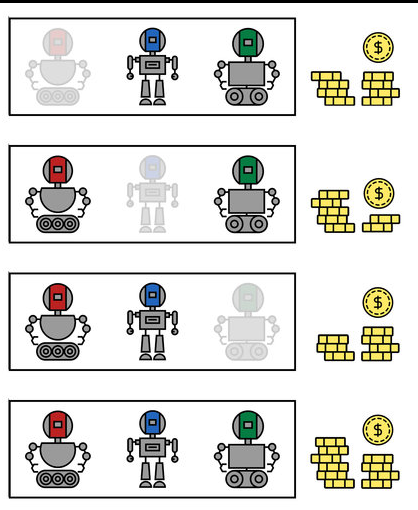
\includegraphics[scale=0.3]{./images/Shap_coal_2.png}
\caption{Rewards without chosen players.}
\end{figure}

However, such an approach does not take into account the fact that some subgroups might have an "emergent" value, i.e., they can give a much bigger (or much worse) value together than separately. It can be that the green robot vibes perfectly with the blue robot, but it is completely useless alone. If the green robot copes well only in group, it would be reasonable to give him a large part of the final reward. That is why we should take into account all the possible coalitions (see figure \ref{rewards_all}).

\begin{figure}[H]
\centering
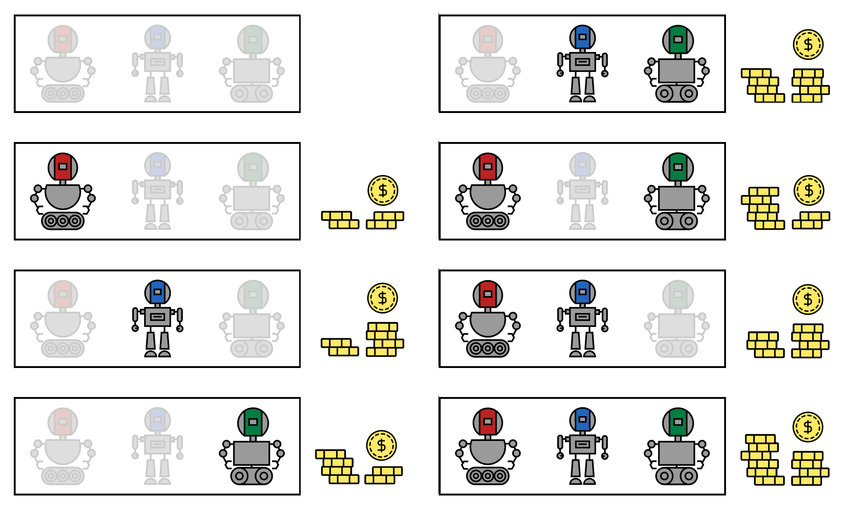
\includegraphics[scale=0.3]{./images/Shap_all_coal.png}
\caption{Rewards of all coalitions.}
\label{rewards_all}
\end{figure}

Shapley values are computed with a skillful formula that uses the rewards obtained by all the possible coalitions.
Shapley values satisfy some natural axioms such as symmetry and "dummy player" (a player who gives nothing receives nothing).
\todo[inline]{\emph{Additivity} to najważniejszy aksjomat, także o nim bym wspomniał; jak mówimy o uniqueness to lepiej wymienić wszystkie żeby uniknąć nieporozumień: additivity, symmetry, efficiency, and nullity. Ja to bym w ogóle definiował aksjomatycznie a wzór przedstawiał jako twierdzenie, ale to już kwestia gustu.}
It guarantees the above-mentioned "fairness" of this method. Moreover, Shapley values are unique to satisfy these axioms [CITE]!. 

Before we give the definition, let us introduce some notation. Let $X$ be the set of players, $v: 2^X \rightarrow \mathbb{R}$ be a function (called coalitional game). We interpret the value $v(S), S \subseteq X$ to be the worth of the coalition $S$.

The exact formal definition is as follows.

\begin{defi}\label{shap_def}
  For the set of players $X$ and the coalitional game $v$ the Shapley value for the player $i$ is:
  \begin{equation*}
      \phi_i(v) = \sum_{S\subseteq X\backslash \{i\}} \frac{|S|!(|X|-|S|-1)!}{|X|!}\left(v(S \cup \{i\}) - v(S)\right).
  \end{equation*}
\end{defi}

In the standard Machine Learning setup, $X$ is the set of tokens (like words in NLP or patches in Computer Vision) and $v$ is for instance the classification model. Shapley values show how important given features are for the model's prediction. One of the important issues with the application of Shapley values is the way of defining $v(S)$ in the above definition. It is not always straightforward how to define the value of the coalition, or, to be more specific, how to mask-out those tokens in the input that we wish to be absent. For the NLP tasks, we can simply ignore the words not belonging to $S$, but when the input is an image, it is necessary to put something in place of the "omitted" patch in order to match the dimensions of the model input. One possible solution is zeroing-out the patches not belonging to $S$. However, this can lead to the problem of out-of-distibution (see section [CITE]! below). While the model was originally trained to fit the data on some high-dimensional manifold, putting zeros throws the input away from this manifold which can yield unexpected behavior of the model.



If we denote the number of players by $n$ then the number of all possible coalitions is $2^n$. Therefore, it is infeasible to consider all the possible coalitions, even for small $n$. It creates the need of some faster approximations with speed-accuracy trade-off.


In the field of XAI, Shapley values are referred to as a model-agnostic method of explanation since it does not take into account any specific properties of the considered model. It takes only the outputs of the model, no matter how they are generated. However, when we use approximation techniques, Shapley values can depend on the model architecture as we will see in Chapter \ref{r:experiments}. Here we introduce two sparse transformer models which we compare with vanilla transformer architecture during the experiments.







\section{Sparse transformers}
Transformer \cite{DBLP:conf/nips/VaswaniSPUJGKP17} is a deep learning model that was originally proposed as a sequence-to-sequence model \cite{DBLP:conf/nips/SutskeverVL14} for machine translation. The main advantage of transformers over previous state of the art RNN or LSTM models is their ability to capture long-range dependencies in the input sequences. While RNN and LSTM process the input sequentially, transformers manage all the input sequence simultaneously \cite{DBLP:journals/corr/abs-2306-07303}.
Besides language related applications, transformers turned out to be successful also in computer vision \cite{DBLP:conf/iclr/DosovitskiyB0WZ21} or audio processing \cite{DBLP:journals/corr/abs-2106-04554}. 

Transformer is the sequence-to-sequence model divided into encoder and decoder models. Each of them is a stack of $L$ identical blocks. The encoder consists of multi-head self-attention module, which is the core element of transformer and a linear layer on top of it. Decoder has a similar architecture. Apart from the encoder components, it inserts a sub-layer that performs the self-attention over the output from the encoder. Another modification is masking, which prevents the decoder from attending to subsequent positions. It ensures that predictions for the $i$-th token depend only on the previous tokens. The overall architecture of the vanilla Transformer architecture is given in figure \ref{attention}.

\begin{figure}[H]
\centering
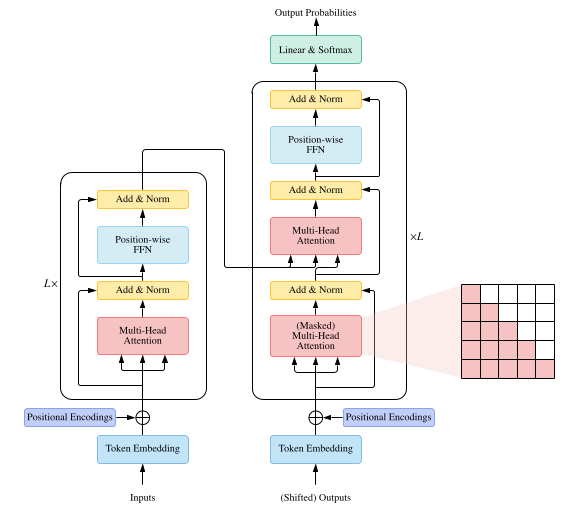
\includegraphics[scale=0.5]{images/attention.png}
\caption{The vanilla Transformer architecture.}
\label{attention}
\end{figure}


The core component of the Transformer architecture is the attention module, which can be defined as follows.

\begin{defi}\label{attention_def}
    Let $Q \in \mathbb{R}^{N\times D_k}$, $K \in \mathbb{R}^{M\times D_k}$ and $V \in \mathbb{R}^{M\times D_v}$ be matrices. The scale dot-product attention is given by
        \begin{equation*}
        \normalfont
        \textrm{Attention} \left( Q, K, V \right) = \textrm{softmax}\left(\frac{QK^T}{\sqrt{D_k}} \right) V.  
    \end{equation*}

\end{defi}

The matrices $Q, K, V$ are referred to as queries, keys, and values, respectively. Queries and keys are responsible for determining which values to attend. The most important values are those for which queries and keys are similar, i.e., have a big dot product. They are in addition bumped up by the softmax function. The scaling factor $\frac{1}{\sqrt{D_k}}$ serves to counteract the effect that the dot product of $Q$ and $K$ grows large, pushing the softmax function into regions where it has extremely small gradients \cite{DBLP:conf/nips/VaswaniSPUJGKP17}.

Instead of performing a single attention, it turned out to be beneficial to stack several attentions in parallel (see Figure \ref{multi-head}). Such multi-head attention allows the model to attend information from different representations of the input. Experiments conducted in \cite{DBLP:conf/nips/VaswaniSPUJGKP17} showed that different heads learn to perform different tasks.

\begin{figure}[H]
\centering
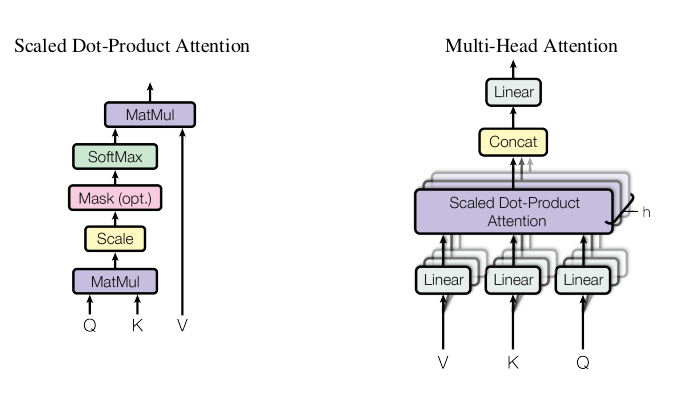
\includegraphics[scale=0.7]{images/attention_module.png}
\caption{Scale-dot product attention (left) and Multi-head attention which consists of several stacked attention layers.}
\label{multi-head}
\end{figure}



Since Transformer has become the go-to architecture for various tasks, a variety of its variants (a.k.a. X-formers) have been proposed (see \cite{DBLP:journals/corr/abs-2106-04554} where was proposed a taxonomy of X-formers). One of the most important challenges of applying Transformer is its relative inefficiency. Indeed, Transformer uses all query-key pairs which gives quadratic complexity in the length of the input. There have been proposed numerous methods to avoid this issue \cite{DBLP:journals/csur/TayDBM23}. In our task to analyse the interpretability of sparse transformers we have chosen two of them.

\chapter{Used models}\label{r:sparse_transformers}

The quadratic complexity of Transformer occurs in the matrix multiplication $QK^T$, i.e., during the comparison of each query with each key. One of the main methods to get along with this problem is to avoid this heavy multiplication by forcing only restricted query-key pairs. Many approaches restrict the attention only to some predefined local neighborhood \cite{DBLP:conf/icml/ParmarVUKSKT18}. Somewhat more advanced approaches limit the field of attention view to some patterns, either fixed or learnable \cite{DBLP:journals/csur/TayDBM23}. Such an approach was used in the Swin model \cite{DBLP:conf/iccv/LiuL00W0LG21} which we will describe later \ref{r:swin}.

Another popular method is to avoid costly matrix multiplication $QK^T$ and instead multiply first keys by values ($K^TV$) and only then by queries ($Q(K^TV))$. Due to the softmax operation on the result of the multiplication $QK^T$ we cannot simply change the order, but it is feasible by viewing the attention mechanism through kernelization. Kernels enable us to omit the softmax operation by introducing other matrices, which allow us to represent the result of the attention mechanism as the product of some other matrices: $Q', K'$ with the same $V$. This approach was applied in Performer \cite{DBLP:conf/iclr/ChoromanskiLDSG21} which we will describe in more detail now.


\section{Performer}\label{r:performer}


The key component of the Performer's architecture is \todo{the} FAVOR+ mechanism (\textit{Fast Attention Via positive Orthogonal Random features}), a new method for approximating softmax and Gaussian kernels. The standard attention can be presented in the following way:
\begin{equation}
    \textrm{Attn}(Q, K, V) = D^{-1}AV, \; A=\textrm{exp}\left(QK^T/\sqrt{d}\right), \; 
    D = \textrm{diag}\left(A1_{L}\right).
\end{equation}\label{attention_equation}

Here the matrix $D$ is introduced instead\todo{in place of the} of softmax denominator in order to have a more convenient form of the attention matrix $A$. The quadratic complexity comes from the fact that we have to apply the exponent function to the product of $Q$ and $K^T$. If we could replace the exponent by some linear function, we could multiply $K^T$ with $V$ first and thus reduce the multiplication cost\todo{See Figure \dots}. That is where the kernels come in. 


\begin{figure}[H]
\centering
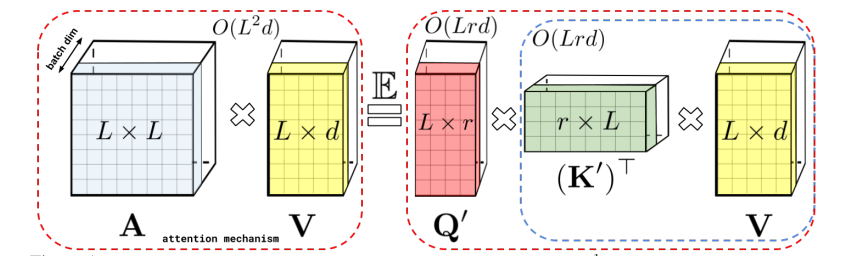
\includegraphics[scale=0.5]{./images/performer.png}
\caption{In the standard attention mechanism (on the left) we first get the $L\times L$ matrix with quadratic time complexity and then have to multiply it by $V$ also with quadratic time. Performer adopts kernels to change the multiplication order and reduce the time complexity to linear.}
\end{figure}




Kernels are functions which are the scalar products in some another space. More specifically, let $\phi : \mathbb{R}^d \rightarrow \mathbb{R}^r_+$ be a randomized mapping and $x, y \in \mathbb{R}^d$. Then we define the kernel $K:\mathbb{R}^d \times \mathbb{R}^d \rightarrow \mathbb{R}_+$ as:
\begin{equation}
    K(x,y) = \mathbb{E} \left[\phi(x)^T\phi(y)\right].
\end{equation}\label{kernel_def}
In our case we have a matrix $A$ as defined in \ref{attention_equation} which we would like to linearize in some way. We define the function $K:\mathbb{R}^d \times \mathbb{R}^d \rightarrow \mathbb{R}_+$ as:
\begin{equation}
    K(q_i^T, k_j^T) = A(i,j) = \textrm{exp}\left(q_i k_j^T/\sqrt{d}\right).
\end{equation}\label{kernel_attention}
If there exists such a probabilistic space and random maps $\phi$ in this space such that the equation \ref{kernel_def} holds, then we could put the matrix $V$ in the attention definition \ref{attention_def} inside the expected value and multiply $\phi(k_j^T)$ by the matrix $V$ and only then by $q_i$. That is the "FA" (\textit{Fast Attention}) part of the FAVOR+ acronym.


MOŻE JESZCZE COŚ O TYM, ŻE ZWYKLE KERNELE STOSUJE SIĘ W DRUGĄ STRONĘ?

Not every kernel which satisfies \ref{kernel_attention} is suitable for approximation. If we use, for instance, trigonometric functions, it leads to unstable behavior and big variance, especially when kernel scores are close to zero (which is the case for $A$ because many of its entries correspond to tokens of low relevance). It is the case if we take:
\begin{equation}
    \phi(x) = \frac{\textrm{exp}(||x||^2/2)}{\sqrt{m}}\left(sin(\omega _1^T x), \ldots, sin(\omega _m^T x), cos(\omega _1^T x), \ldots, cos(\omega _m^T x)\right),
\end{equation}\label{trigonometric_kernel}
where $\omega _1, \ldots \omega _m \stackrel{\textrm{i.i.d.}}{\sim} \mathcal{N}(0, I_d)$. Note that we can choose both the mapping $\phi$ and its output dimension $2m$ to better approximate the matrix $A$. In Lemma 2 from \cite{DBLP:conf/iclr/ChoromanskiLDSG21} it is proven that although the kernel given by \ref{trigonometric_kernel} is unbiased, its variance tends to infinity as approximated values tend to 0.


That is why the \textit{positive random features} were introduced. Positive random features are given by the random map feature:
\begin{equation*}
    \phi(x) = \textrm{exp}\left(\omega^T x-\frac{||x||^2}{2}\right),
\end{equation*}
where $\omega \sim \mathcal{N}(0, I_d)$, which is positive due to the exponent. Since the kernel is the expected value of random maps $\phi$, in practice we have to sample from the normal distribution. In order to even further reduce the variance we can apply Gram-Schmidt orthogonalization procedure to the sampled $\omega_1, \omega_2, \ldots, \omega_m$. This step requires $m\leq d$, that is the number of samples has to be smaller than the embedding dimension, which was always the case in \cite{DBLP:conf/iclr/ChoromanskiLDSG21}.

\section{T2T\textunderscore ViT}\label{s:T2T}

T2T\textunderscore ViT \ref{0007DBLP:conf/iccv/0007CWYSJTFY2121} is a visual transformer that is based on the Performer backbone and uses a special tokens-to-token (T2T) tokenization module. This technique can model the local structure information of surrounding tokens and reduce the length of tokens iteratively, replacing many tokens with only one. The vanilla vision transformer splits each image into a sequence of tokens without taking into account their spatial order. It was argued in \ref{0007DBLP:conf/iccv/0007CWYSJTFY2121} that this simple tokenization hinders modeling of the local structure. Although ViT achieves the satisfactory performance on benchmarks, it is difficult to train it from scratch, and this training requires a lot of data, because ViT is not prepared to model the local structure and has to learn it somehow from scratch. The Tokens-to-Token module aims to overcome this issue by recursively aggregating neighboring tokens into one token. The main idea and the standard block of the T2T\textunderscore ViT architecture is shown on the Figure \ref{im: T2T architecture}.

\begin{figure}[H]
\centering
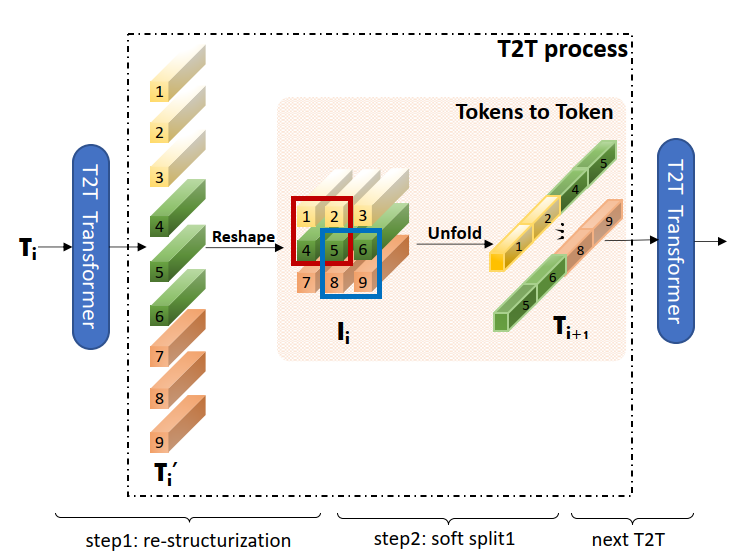
\includegraphics[scale=0.6]{./images/T2T_ViT_architecture.png}
\caption{T2T\textunderscore ViT basic block. Source: \cite{0007DBLP:conf/iccv/0007CWYSJTFY2121}}.
\label{im: T2T architecture}
\end{figure}


The Tokens-to-Token module is used between two transformer layers and is the core of the architecture. It consists of two phases:
\begin{itemize}
	\item \textbf{Re-structurization} Given the output from the transformer layer, it is transformed as an image into a spatial representation.
	\item \textbf{Soft Split} When we have the spatial representation, we unfold so that neighbors are in one token. The unfold operation is performed after each reshaping in the Tokens-to-Token module and at the very beginning of the model, when the image itself is unfolded. In Figure \ref{im: T2T architecture}, the tokens 1, 2, 4, 5 which are close to each other on the image, become one token after the Soft Split operation. With this operation, we not only aggregate the local information from surrounding pixels and patches but also reduce the number of tokens. In order to avoid information loss, the patches that are unfolded overlap. In this way is created a prior that patches close to each other have a bigger correlation.

\end{itemize}





\section{Swin}\label{r:swin}
The Swin model (\textbf{S}hifted \textbf{win}dow) \cite{DBLP:conf/iccv/LiuL00W0LG21} limits the computations related to the attention matrix by the window-based approach. Self-attention is calculated only on some subsets of neighbouring patches (windows) rather than on the whole image. If we choose the window size to be constant, then the complexity is reduced to linear on the number of patches.
\todo{Wymazać ``ours'' z obrazka}
\begin{figure}[H]
\centering
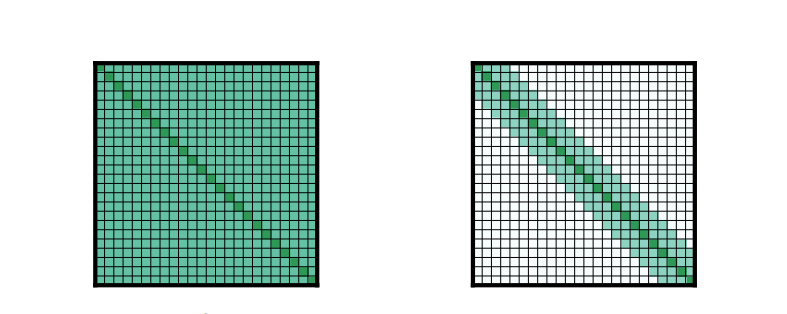
\includegraphics[scale=0.4]{./images/sliding_window.png}
\caption{In the full self-attention (left) pattern each token attends to each other while for the window approach (right) tokens attend only to their neighbourhoods. Source: \cite{DBLP:journals/corr/abs-2004-05150}}.
\end{figure}


A straight-forward solution in this window-based framework could be a pattern where each token attends only to a fixed number of neighbouring tokens $w$. Such an approach was used in Longformer \cite{DBLP:journals/corr/abs-2004-05150}. Complexity of this pattern is $O(w \times n)$, where $n$ is the number of tokens, so constant 
value of $w$ gives the linear complexity. 

There is, however, a caveat to this method, since pixels lying far from each other do not appear together in any window. In order to provide some connections across windows in \cite{DBLP:conf/iccv/LiuL00W0LG21} was proposed a shifted window partitioning approach (see figure \ref{changing_windows}. 


\begin{figure}[H]
\centering
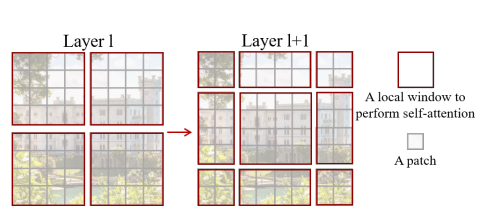
\includegraphics[scale=0.6]{./images/changing_windows.png}
\caption{In the Swin model, the self-attention is computed only within local windows, which vary in consecutive layers.}
\label{changing_windows}
\end{figure}

As the name suggests, this approach consists of a shifting window when attention is computed. Thus, at each layer, the tokens attend to other tokens. Moreover, since windows are shifted by half of their size, there is much space in common, which gives some connections between far tokens. 

To finally improve performance, Swin Transformer constructs hierarchical feature maps like feature pyramid network \cite{DBLP:conf/cvpr/LinDGHHB17} or U-Net \cite{DBLP:conf/miccai/RonnebergerFB15}. 

\begin{figure}[H]
\centering
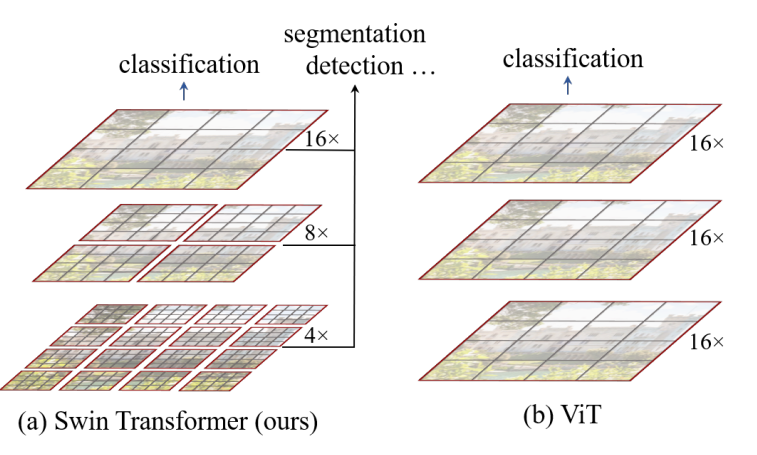
\includegraphics[scale=0.3]{./images/Swin_window.png}
\caption{Swin model (a) computes self-attention only within each local window. On the other hand, standard ViT (b) uses self-attention on the entire image.}
\end{figure}

Swin Transformer proceeds from small windows consisting of small patches up to one big window with bigger patches. Window size increases together with the size of patches which are merged from smaller patches. In this way, the number of tokens in self-attention can remain constant.







\chapter{Shapley Values for Visual Transformers}\label{r:visual_shap}
Since its first usage in computer vision in
\cite{DBLP:conf/iclr/DosovitskiyB0WZ21}, Transformer has become the state of the art model also in this domain. Thus, it became urgent to provide some technique for explanation of transformers applied to images. At first glance, it might seem that attention is self-explanatory, as attention values can indicate the importance of features. However, recent works (\cite{DBLP:conf/acl/SerranoS19},
\cite{DBLP:conf/cvpr/CheferGW21}) raised questions about the validity of attention values as an explanation. It was shown that this method provides an incomplete picture of a model's dependence on each token as it takes into account only the attention component in the sequence of the model's operations. The attention component taken apart provides an incomplete picture of the model's dependencies.

That is why there is a need for another solution, and Shapley values come in as a theoretically grounded explanation method. The main drawback of this method is its computational cost, since it has exponential time in the number of players, which in the context of computer vision are patches. In \cite{DBLP:conf/iclr/Covert0L23}, a method was proposed to efficiently estimate Shapley values for vision transformers. This method generates Shapley value explanations via a separate, learned explainer model. In the following chapter we will describe this approach in more detail.



\section{Surrogate model}\label{s:surrogate}
Shapley values are the removal-based explanation, i.e. they measure the feature importance by removing features and checking how the prediction changes. In the context of computer vision, features are patches so to compute the Shapley value of a computer vision model we need to remove the chosen patches from the image. 

Using self-attention operation we can remove patches in an elegant way. We can ignore the chosen patches by masking them in the attention operation. This approach is similar to the causal attention in transformer language models like GPT-3 \cite{DBLP:conf/nips/BrownMRSKDNSSAA20}.

Another approach could be to set some patches to zero or average the prediction across randomly sampled replacement values. As it was shown in \cite{DBLP:conf/nips/NaseerRKHKY21}, ViTs are highly robust to occlusions. It means that simple zeroing out of the patches does not degrade much the model performance.  Given a ViT model $f$, we can evaluate it on a masked input $\mathbf{x_s}$. However, it leads to the off-manifold problem: the model $f$ was trained only on full images and masked images are out of the learned data distribution \cite{DBLP:conf/aistats/TaufiqBM23}.  To manage this problem there was introduced a surrogate model \cite{DBLP:conf/iclr/FryeMBCSF21}. It is trained on masked images to imitate the outputs of the original model on unmasked images. If $\mathbf{x}$ is the original image and $\mathbf{x_s}$ is the image with masked patches from the set $s$, then we train the model $g(\mathbf{x_s})$ to have the nearest possible output to the output of $f(x)$. More formally, we fine-tune the model $g$ using the following loss:
\begin{equation*}
    \textrm{min}_{\beta} \mathbb{E}_{p(x)} \mathbb{E}_{p(s)} \left[D_{\textrm{KL}} \left(f(\mathbf{x};\eta) || g(\mathbf{x_s};\beta)\right)\right],
\end{equation*}
where $p(s)$ is the distribution over subsets. This loss has a theoretical guarantee that the optimal solution $g(\mathbf{x_s};\beta*)$ satisfies the property:
\begin{equation*}
    g(\mathbf{x_s};\beta*) = \mathbb{E}\left[f(\mathbf{x};\eta) || \mathbf{x_s}=x_s \right],
\end{equation*}
i.e. the optimal model $g(\mathbf{x_s})$ outputs the expected prediction given the available information about unmasked input $x$. With such a model we are able to provide more robust and trustworthy model outputs on the masked images. It is needed both for computing the Shapley values from scratch and for the explainer model.

\section{Model for Shapley values computation}\label{s:model}
Using surrogate model we can introduce the coalitional game $v_{xy}(s) = g_y(x_s;\beta)$, where $y$ is one of the classes and $s$ some subset of image patches. Instead of training a neural network on some ground truth Shapley values one can use an optimization-based characterization of the Shapley value 

[CITE! Charnes et al. 1988 (Extremal Principle Solutions of Games in Characteristic Function Form: Core, Chebychev and Shapley Value Generalizations)]

This characterization allows to find the Shapley values by minimizing the following objective introduced in \cite{DBLP:conf/iclr/JethaniSCLR22}:
\begin{equation}
    \begin{split}
        \mathcal{L}(\theta) &= \mathbb{E}_{p(x,y)} \mathbb{E}_{p(s)}  \left[\left(v_{xy}(\mathbf{s})-v_{xy}(\mathbf{0} -\mathbf{s}^T \phi _{ViT}(\mathbf{x},\mathbf{y};\theta)\right)^2\right] 
        \\
        &    \textrm{s.t.  } \mathbf{1}^T \phi _{ViT}(x,y;\theta) = v_{xy}(\mathbf{1}) - v_{xy}(\mathbf{0}) \textrm{    for all   } x,y,
    \end{split}
\end{equation}\label{explainer_loss}
where $p(\mathbf{s})$ is a distribution defined as $p(s) \propto (\mathbf{1}^Ts - 1)! (d - \mathbf{1}^Ts -1)!$ for $0 < \mathbf{1}^Ts < d$ and $p(\mathbf{1}) = p(\mathbf{0}) = 0$ and $\phi _{ViT}$ is the explainer model which takes image and target class as input and outputs the approximate Shapley values in a single forward pass. Compared to the definition of Shapley values \ref{shap_def}, the probability distribution $p$ accounts for the fraction with factorials and the crucial part is the fact that there is no sum over all possible coalitions. It is crucial, because the number of coalitions ($2^n$ is what makes the computation of Shapley values so expensive. In one pass, $\phi _{ViT}$ approximates in some sense only $v_{xy}(\mathbf{s})-v_{xy}(\mathbf{0})$, i.e. the profit of taking players from the set $s$ to the coalition. The explainer model needs for training only a pretrained surrogate model. Using it, we can define the loss \ref{explainer_loss}




\chapter{Experiments}\label{r:experiments}
We conduct experiments on CIFAR-10 and HyperKvasir, which is the largest available gastrointensinal dataset. Both sets are well-suited to the task of explanation because they have quite easily observable important patches which we expect to be marked as such by explanation techniques. CIFAR-10 is a well known dataset with everyday life classes such as car, bird, cat, dog, and truck. HyperKvasir is a more specialistic dataset that contains gastrointestinal images with some disabilities. As is often the case with the medical data, some findings occur more frequently than others, which makes the data classes imbalanced. To overcome this issue, we have chosen 1000 images with polyps and 1000 images without polyps. In this way, we were able to train more reliable classifier models. 

A considerable advantage of the HyperKvasir dataset is that it provides some ground truth for explanation. Together with images there are segmented images with assigned anomalies. Therefore, explanations will give us information on whether the model predictions are based on patches where anomalies indeed appear or whether the model takes random or arbitrary features, like was the case with the famous husky misclassification example (see figure \ref{husky}).

\begin{figure}[H]
\centering
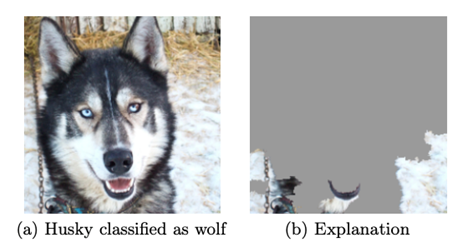
\includegraphics[scale=0.5]{./images/husky.png}
\caption{The explanation showed that the model did not even take into account the husky face but only the "wild" background.}
\label{husky}
\end{figure}


We present in the Figure \ref{polyps_segmentation} the example polyps together with their ground-truth segmentation masks.


\begin{figure}[H]
\centering
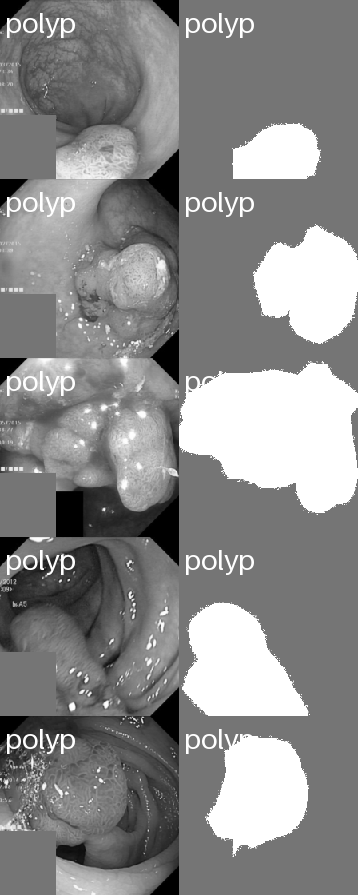
\includegraphics[scale=0.5]{./images/polyps_segmentation.png}
\caption{Polyps with their segmentation masks}
\end{figure}

In the further experiments we will use these segmentation masks to analyze the explanations of the models for the polyp class (see Section \ref{s:HyperKvasir Explanations} below).



The overall experiments were conducted in three stages. At first, we trained classification models on the unchanged data. Then we trained surrogate models, which are classification models on the masked data. Surrogate model is required for training of the explainer model which explains surrogate predictions giving approximations of Shapley values.

For both classifier and surrogate models, we used batch size $64$, learning rate $5e-5$, and AdamW optimizer. The explainer model requires more hyperparameters. The most important of them is freeze\textunderscore backbone, which decides how many layers to freeze from the explainer backbone. It was noted in \ref{DBLP:conf/iclr/Covert0L23} that ViTs are difficult to train, and we find that fine-tuning is important to train the explainer effectively. We performed experiments to verify which freezing strategy works best. We took into consideration three options: freeze all the layers, freeze all the layers except the last two, and no freezing. We found out that the last option, being the slowest, gave the best results.

Overall, we trained 6 classifier models (3 model types, 2 datasets), 12 surrogate models (3 model types, 2 datasets, and 2 number of players: either 16 or 196), and 48 explainer models (3 explainers to explain each of 12 surrogate models).


\section{Image classification on CIFAR-10 and HyperKvasir}

For image classification we used two sparse transformers (Swin and Performer) described in \ref{r:sparse_transformers} pretrained on ImageNet dataset. We used also the plain Visual Transformer (ViT) \cite{DBLP:conf/iclr/DosovitskiyB0WZ21}. In later sections we will focus on differences between ViT and sparse transformers both in terms of performance and interpretability. 

For the training we used the standard augmentation techniques like RandomResizedCrop, RandomHorizontalFlip or RandomRotation. HyperKvasir images had to be resized to fit the models' input size $(224\times 224)$. 

The accuracy results of transfer learning are given below.
\\


\begin{center}
\begin{tabular}{clSSSSS}
\toprule
% \multicolumn{2}{c}    {Trained Data}    &   

& Model&  {HyperKvasir} &   {CIFAR-10} \\

\midrule
                &   ViT         &   90.5    &   97.7\\
                &   T2T\textunderscore ViT       &   93.7    &   97.7\\
                &   Swin      &   91.3    &   98.0\\
\midrule

\bottomrule
\end{tabular}
\end{center}


\section{Surrogate models}
In section \ref{s:surrogate} we briefly introduced surrogate models and explained why it is useful to additionaly train them. Here we provide the results together with more details. 

Surrogate model is the classification model trained on the masked inputs to resemble the outputs of the model trained without masking. To train the surrogate model we need to prepare the masked data.
We have two masking approaches, each of them having its drawbacks and advantages. For both datasets (CIFAR-10 and HyperKvasir) we resize the image to the size $224\times 224$. In the first setup we divide image into $4\times 4$ square patches consisting of $56\times 56$ pixels. In the second setup we divide image into $14\times 14$ square patches consisting of $16\times 16$ pixels. Thus, we have either 16 or 196 players. In the first case we have $2^{16}=65,536$ coalitions. This number is small enough to make feasible the computation of Shapley values from scratch. 

At the beginning, we present the performance of surrogate models. Below are the images from the batch of masked CIFAR-10 images with marked predicted classes (green if correct, red for misclassification). One can notice that all three models make mistakes practically only for the completely or almost completely masked images.




In order to see how the performance was improved due to the additional training on the masked data, we can view similar image grids for the vanilla classifier model. We can see that it makes about two times more mistakes except the swin model for which the surrogate has smaller advantage. This unexpected behavior of the Swin model is reflected also in the accuracy results where the Swin model is the best both for surrogate and the vanilla model.


\begin{table}
\begin{center}
\caption{CIFAR-10 classification results\\}
\begin{tabular}{clSSSSS}
\toprule

% \multicolumn{2}{c}    {Trained Data}    &   

& Model&  {Vanilla unmasked} &   {Surrog unmasked} 
& {Vanilla masked}
& {Surrog masked}
\\

\midrule
                &   ViT         &   97.90    &   98.21  &
                75.03 &
                85.42\\
                &   T2T\textunderscore ViT       &   97.67    &   97.98 &
                74.81 &
                84.79\\
                &   Swin      &   97.96    &   98.11 &
                78.21 &
                86.20\\
\midrule

\bottomrule
\end{tabular}
\end{center}
\end{table}


\begin{table}
\begin{center}
\caption{HyperKvasir classification results}
\begin{tabular}{clSSSSS}
\toprule

% \multicolumn{2}{c}    {Trained Data}    &   

& Model&  {Vanilla unmasked} &   {Surrog unmasked} 
& {Vanilla masked}
& {Surrog masked}
\\

\midrule
                &   ViT         &   90.17    &   90.67  &
                78.17 &
                80.00\\
                &   T2T\textunderscore ViT       &   90.83    &   90.67 &
                71.42 &
                81.92\\
                &   Swin      &   88.67    &   88.00 &
                77.67 &
                81.00\\
\midrule

\bottomrule
\end{tabular}
\end{center}
\end{table}

The overall accuracy of the models on the masked data is shown in figure \ref{masked_accuracy}. Masked \% represents how many patches were averagely masked in the data. Each patch is masked independently with a probability of 50\%. All six models begin at about 97\% accuracy. Vanilla classifiers begin to gradually decrease performance at about 30\% of masked patches, while the surrogates models' accuracy remain almost unchanged. It is only at about 70\% of masked patches that surrogates' accuracy begins to drop.


\begin{figure}[H]
\centering
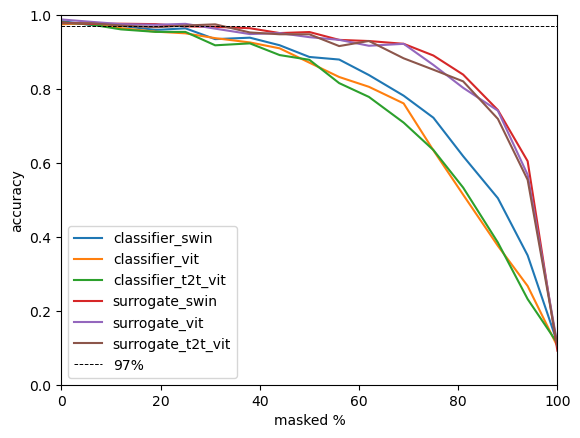
\includegraphics[scale=0.8]{./images/masked_accuracy.png}
\caption{Accuracy of the models with masked patches (CIFAR-10)}
\label{masked_accuracy}
\end{figure}


For the HyperKvasir dataset, the results are much less smooth (see figure \ref{gastro_masked_accuracy}, which is probably due to its smaller size. It is noticeable that the vanilla classifiers are more robust and drop less significantly. It is perhaps because the deciding features of the HyperKvasir are more concentrated and the model predictive power remains almost unchanged until the principal patches remain unmasked.


\begin{figure}[H]
\centering
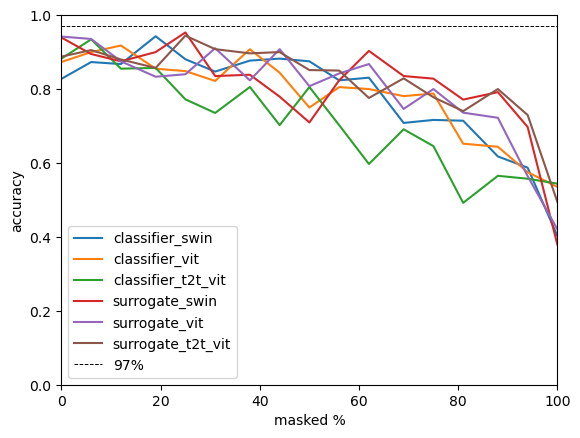
\includegraphics[scale=0.8]{./images/gastro_masked_accuracy.png}
\caption{Accuracy of the models with masked patches (HyperKvasir)}
\label{gastro_masked_accuracy}
\end{figure}










\section{CIFAR-10 Explanations}
In this section we will describe the feature attributions obtained by Shapley values computed from scratch using the formula
  \begin{equation*}
      \phi_i(v) = \sum_{S\subseteq X\backslash \{i\}} \frac{|S|!(|X|-|S|-1)!}{|X|!}\left(v(S \cup \{i\}) - v(S)\right),
  \end{equation*}
where $X$ is the set of players, $i$ is the number of players, and $v$ is the coalitional game. In our case, the coalitional game is defined by the logits of the surrogate model. Due to the strong theoretical guarantees of the Shapley values, we can refer to them as ground-truth explanations. The Shapley values computed directly from the definition indicate where really are the patches essential for the prediction. Therefore, using them, we can verify whether the model reflects commonsense presumptions about the important features. For the CIFAR-10 dataset, we can rely on intuition which says, for instance, that for the animals, the most important feature is their head or, for the plane, its wings. As for the HyperKvasir dataset, we have pixel-level annotations of the important features (polyps), and we can check whether the models' predictions are based on what they should be based on (see \ref{s:HyperKvasir Explanations}).





All the models have rather strong correlation between each other (see Figures \ref{shap_swin_t2t_vit}, \ref{shap_vit_swin}, \ref{shap_vit_t2t_vit}). The strongest correlation occurs between two sparse transformers. It can be seen also in Table \ref{shap_consistency}. We check there how many images get the biggest Shapley value for the same patch. Every pair score is greater than 50\%. It is not surprising that the consistency is not exact because for 16 players, patches are rather small. It means that important features of the image can appear in two patches, and one model can prefer one patch while the other prefers some of its neighbors. It is mostly visible for the class "truck" (see Figure \ref{Truck_shapley}). 

\begin{figure}[H]
\centering
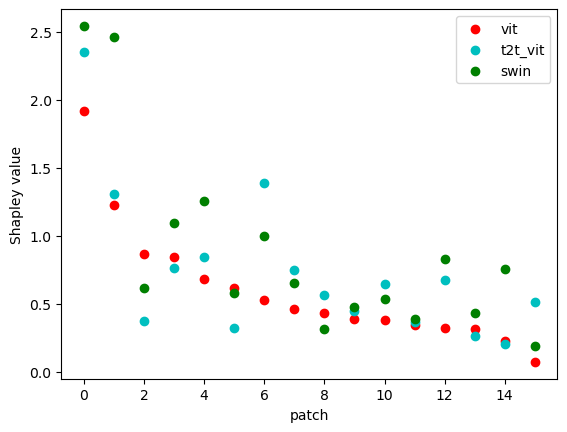
\includegraphics[scale=0.5]{./images/Truck_shapley.png}
\caption{Shapley values for the truck class}
\label{Truck_shapley}
\end{figure}

We plotted several curves, which show the Shapley values for one image and for all 16 patches. The shapes of the curves for different models vary considerably. It is probably due to the fact that the truck has many features, which could lead to the conclusion that there is a truck in the image. There are many indicators of "truckness." On the other hand, the shapes for the "cat" class are almost perfectly consistent (see figure \ref{Cat_shapley}). The reason for this behavior of the models might be that cats are more definite beings than trucks. Models may learn that the most important feature of cat is its head while there are many other important features like legs, trunk, tail. Models assign to each of the features some proportionate importance. The features of the truck are much less sharp. For one model a white patch might enhance the probability of the truck class because it learned that the trucks are often white. For another model the same white patch might work against the truck class as it is rather indicator of the plane.


\begin{figure}[H]
\centering
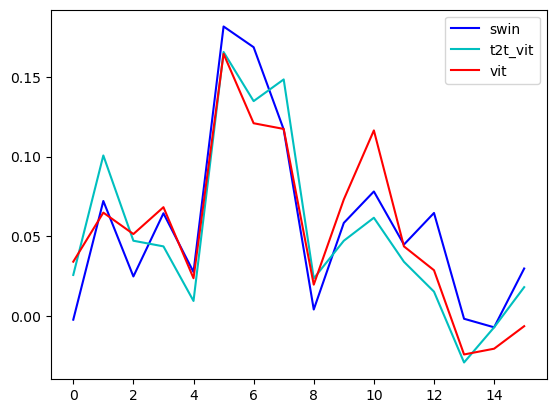
\includegraphics[scale=0.5]{./images/Cat_shapley.png}
\caption{Shapley values for the cat class}
\label{Cat_shapley}
\end{figure}




\begin{figure}[H]
\centering
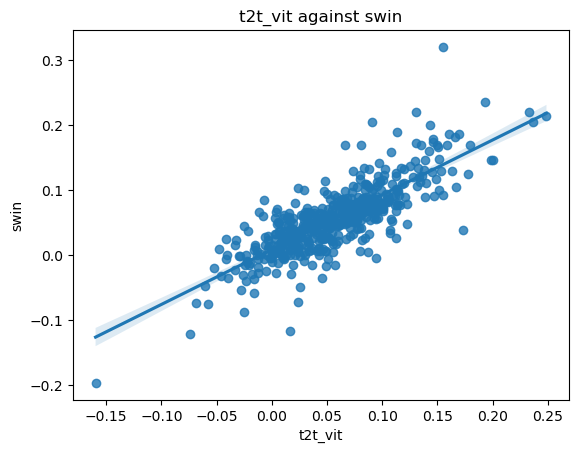
\includegraphics[scale=0.5]{./images/shap_swin_t2t_vit.png}
\caption{Shapley values correlation: Swin and T2T\textunderscore ViT}
\label{shap_swin_t2t_vit}
\end{figure}


\begin{figure}[H]
\centering
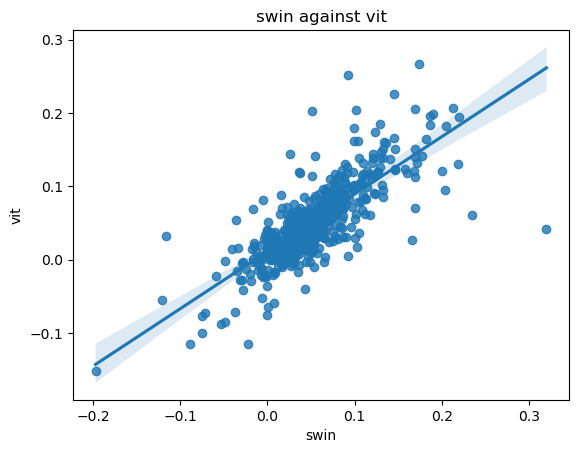
\includegraphics[scale=0.5]{./images/shap_vit_swin.png}
\caption{Shapley values correlation: ViT and Swin}
\label{shap_vit_swin}
\end{figure}


\begin{figure}[H]
\centering
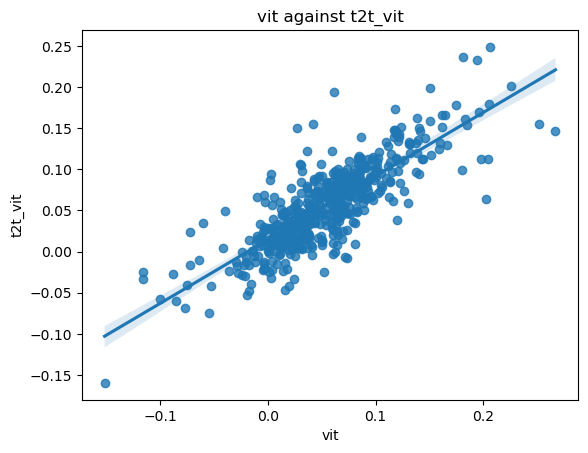
\includegraphics[scale=0.5]{./images/shap_vit_t2t_vit.png}
\caption{Shapley values correlation: ViT and T2T\textunderscore ViT}
\label{shap_vit_t2t_vit}
\end{figure}





\begin{center}
\begin{tabular}{clSSSSS}
\toprule
% \multicolumn{2}{c}    {Trained Data}    &   

& Model & {ViT}  & {T2T\textunderscore ViT} &  {Swin} \\

\midrule
                &  ViT   & 100    &   50.0    &   53.1 \\
                &   T2T\textunderscore ViT       &   50.0    &   100 & 62.5\\
                &   Swin      &  53.1     &   62.5 & 100 \\
\midrule

\bottomrule
\label{shap_consistency}
\end{tabular}
\end{center}



We presume therefore that the Shapley values are more similar for the classes with more definite shapes and features. It can be even better observed in the Figures \ref{vit_shap_grid}-\ref{swin_shap_grid}. For some classes like frog or truck the Shapley values are somehow blurred and there are many patches with a big value (marked as yellow). On the other hand, the classes like cat or bird have quite strict "positive" regions which indicate the importance for the model output.





\begin{figure}[H]
\centering
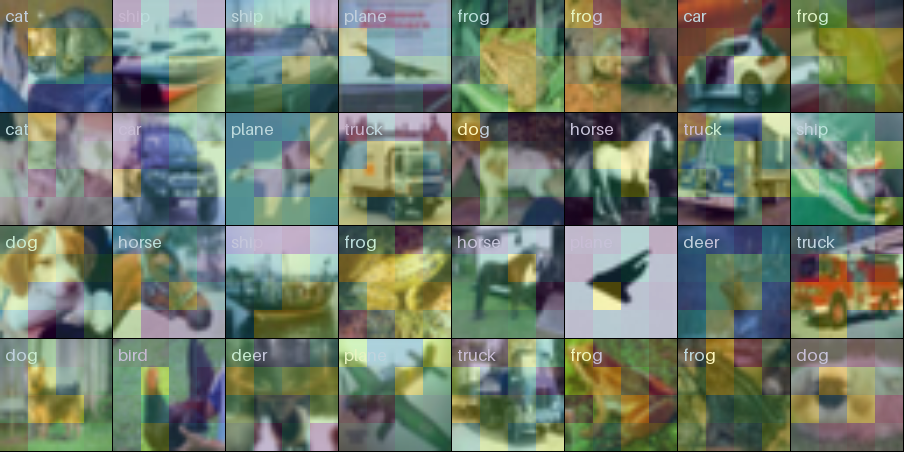
\includegraphics[scale=0.5]{./images/vit_shap_grid.png}
\caption{Shapley values marked on the images for the ViT model}
\label{vit_shap_grid}
\end{figure}


\begin{figure}[H]
\centering
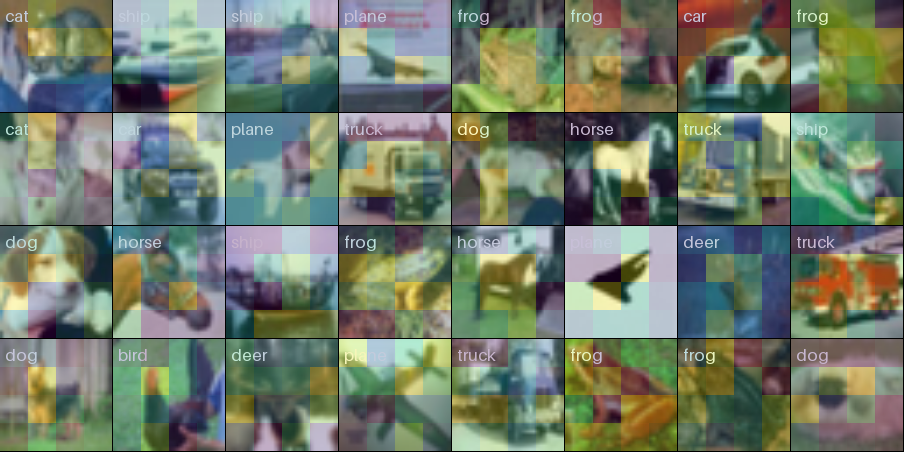
\includegraphics[scale=0.5]{./images/t2t_vit_shap_grid.png}
\caption{Shapley values marked on the images for the T2T\textunderscore  ViT model}
\label{t2t_vit_shap_grid}
\end{figure}


\begin{figure}[H]
\centering
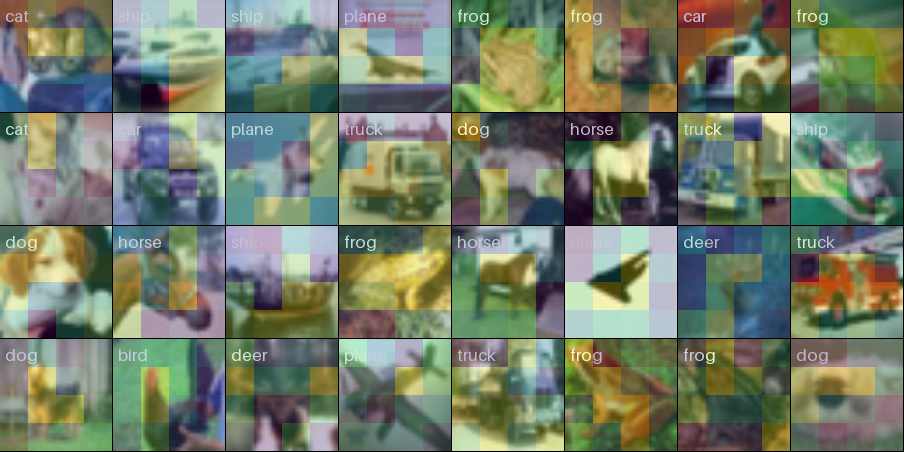
\includegraphics[scale=0.5]{./images/swin_shap_grid.png}
\caption{Shapley values marked on the images for the Swin model}
\label{swin_shap_grid}
\end{figure}



This behavior can be seen in more fine-grained pictures for 196 players (see Figures \ref{vit_shap_grid_196} - \ref{swin_shap_grid_196}). These pictures were produced with the Shapley values computed by the explainer model (see Section \ref{s: model}), because the computation from scratch would require considering each of the $2^{196}$ coalitions. They are compatible with the values computed from scratch for 16 players, i.e., they indicate the same regions of images as important. In the Section \ref{s:evaluation} we will conduct a more thorough evalutation of the explainer model.




\begin{figure}[H]
\centering
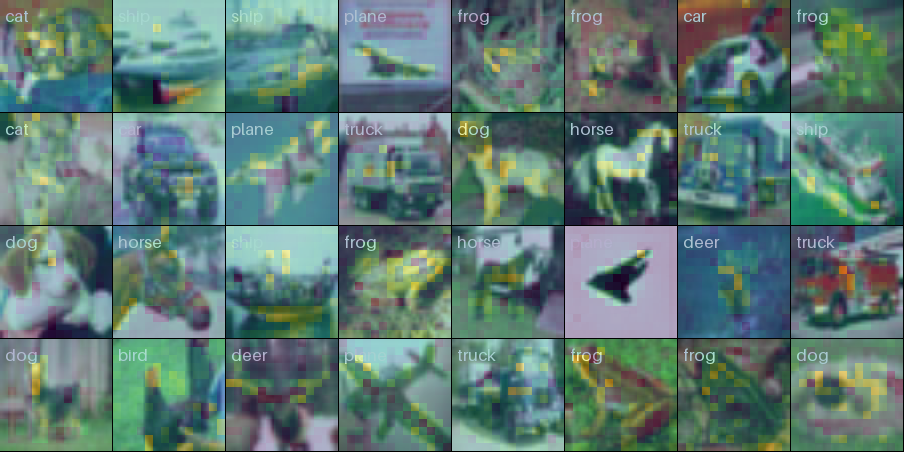
\includegraphics[scale=0.5]{./images/vit_shap_grid_196.png}
\caption{Shapley values marked on the images for the ViT model}
\label{vit_shap_grid_196}
\end{figure}


\begin{figure}[H]
\centering
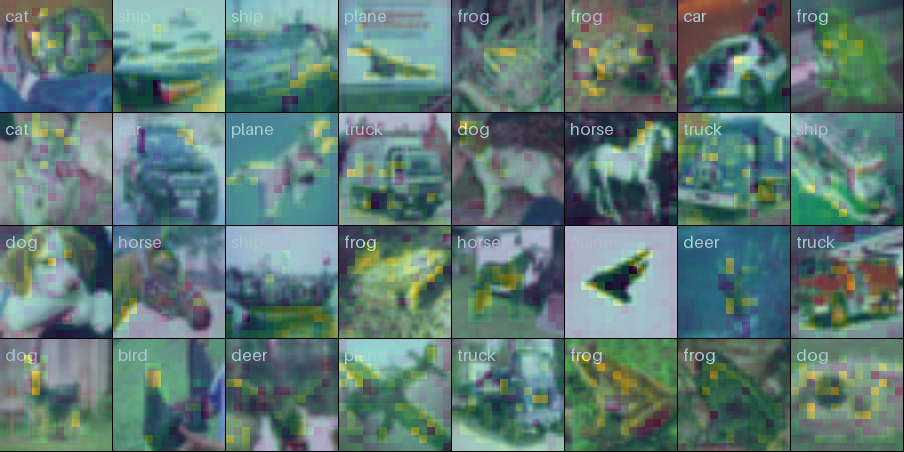
\includegraphics[scale=0.5]{./images/t2t_vit_shap_grid_196.png}
\caption{Shapley values marked on the images for the T2T\textunderscore  ViT model}
\label{t2t_vit_shap_grid_196}
\end{figure}


\begin{figure}[H]
\centering
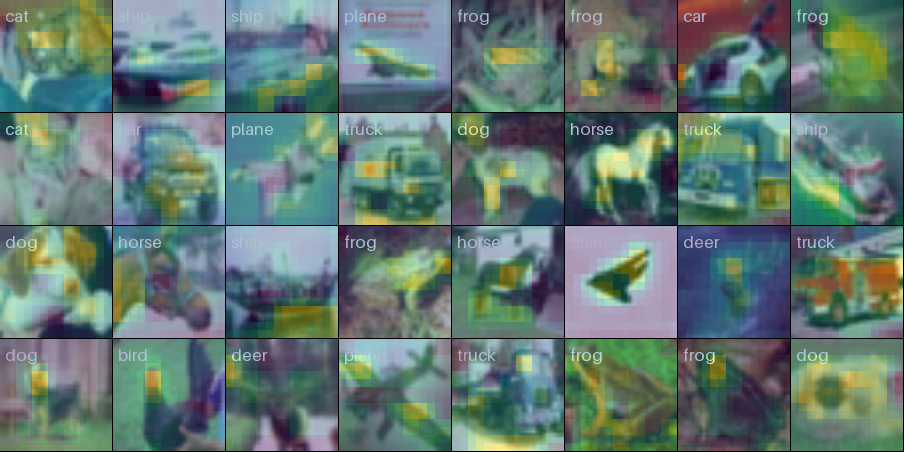
\includegraphics[scale=0.5]{./images/swin_shap_grid_196.png}
\caption{Shapley values marked on the images for the Swin model}
\label{swin_shap_grid_196}
\end{figure}









\section{HyperKvasir Explanations}\label{s:HyperKvasir Explanations}

For the HyperKvasir, we have noticed an interesting issue with the models. Namely, they tended to classify images by some incidental features. Images with polyps and without polyps have another colours, some additional subtitles and edges. The models sometimes pick these properties up. It can be hardly noticed even by a thorough inspection of the models' false predictions on the masked images (see Figure \ref{gastro_vit_masked}) 

\begin{figure}[H]
\centering
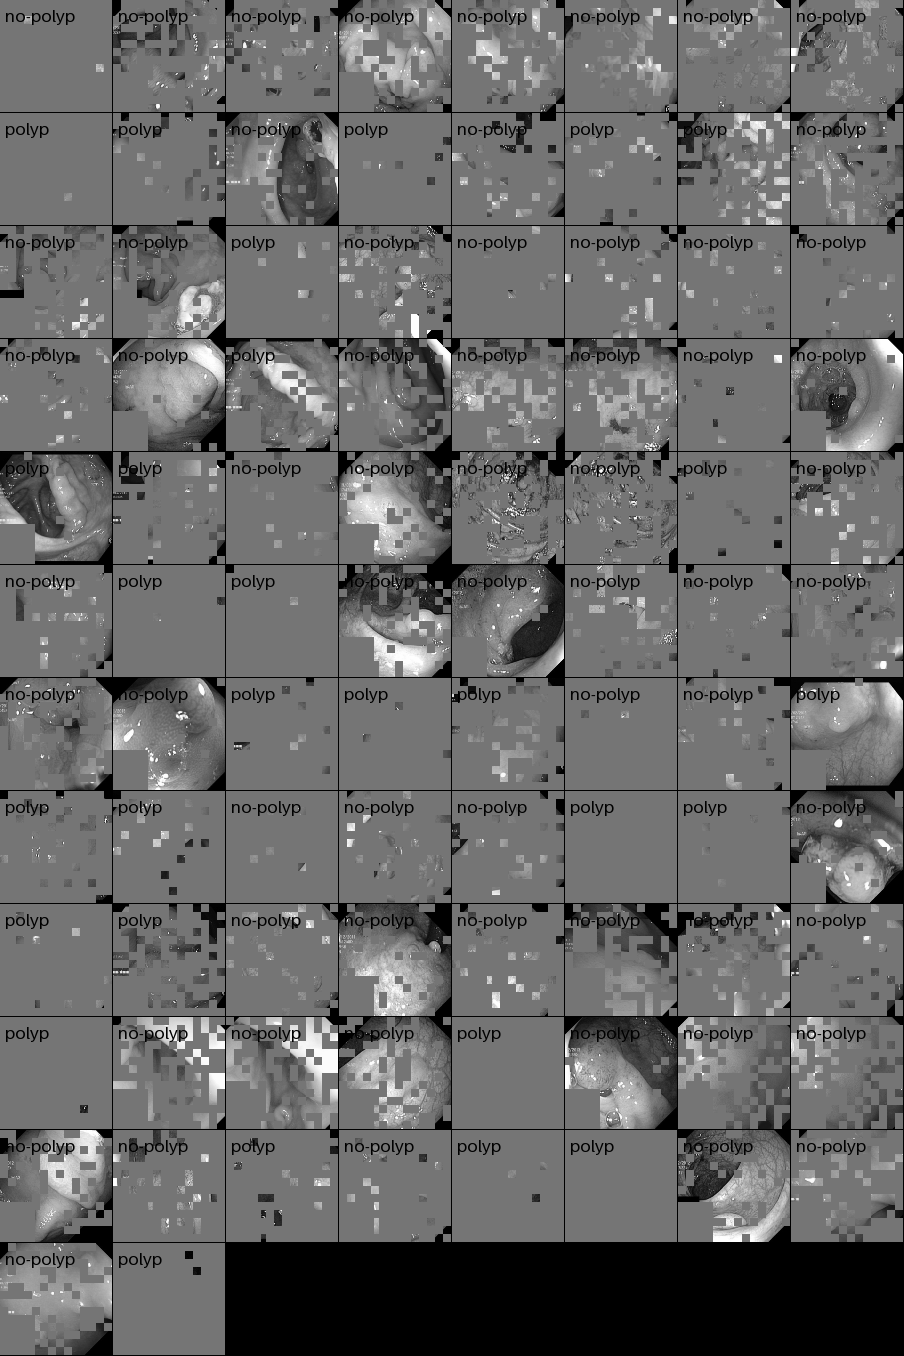
\includegraphics[scale=0.4]{./images/gastro_false_surrogate.png}
\caption{False predictions of the surrogate model}
\label{gastro_vit_masked}
\end{figure}


We can observe that images with fully visible polyps are misclassified when they have masked subtitles or edges. 
However, this unwanted behavior of the model can be seen much more clearly with the Shapley values which indicate explicitly important features. 
(see Figure \ref{Shapley values gastro}). It can be clearly seen that predictions of the surrogate model for the images without polyps are often based on the edges of the image. 

\begin{figure}[H]
\centering
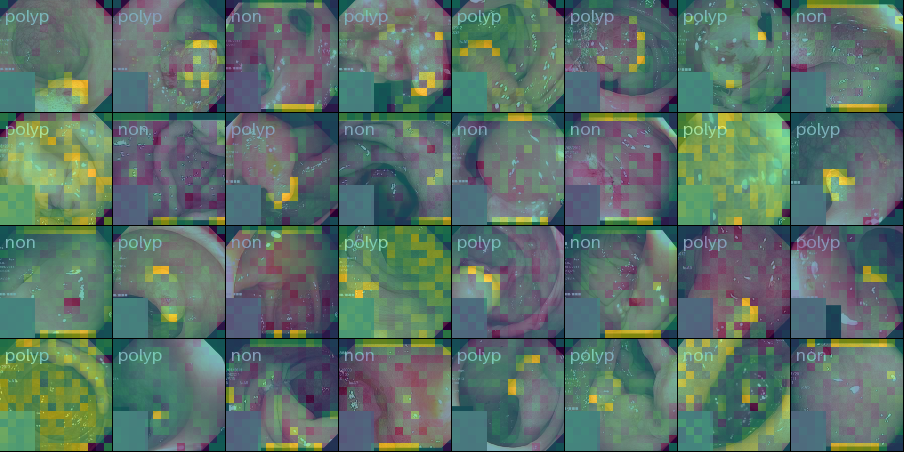
\includegraphics[scale=0.5]{./images/shap_gastro_edges.png}
\caption{Surrogate focuses on incidental features}
\label{Shapley values gastro}
\end{figure}




Here we can see the advantage of Shapley values, which can almost automatically show some problems with the model or with the dataset.
When we noticed the above mentioned issue with the HyperKvasir dataset, we decided to crop the images so that the unwanted additional features would disappear. Indeed, after this operation, Shapley values are the biggest for the regions with polyps and surrogate models focus on the important features as it can be seen on the Figure 
\ref{Shapley values for 196 players cropped gastro}

\begin{figure}[H]
\centering
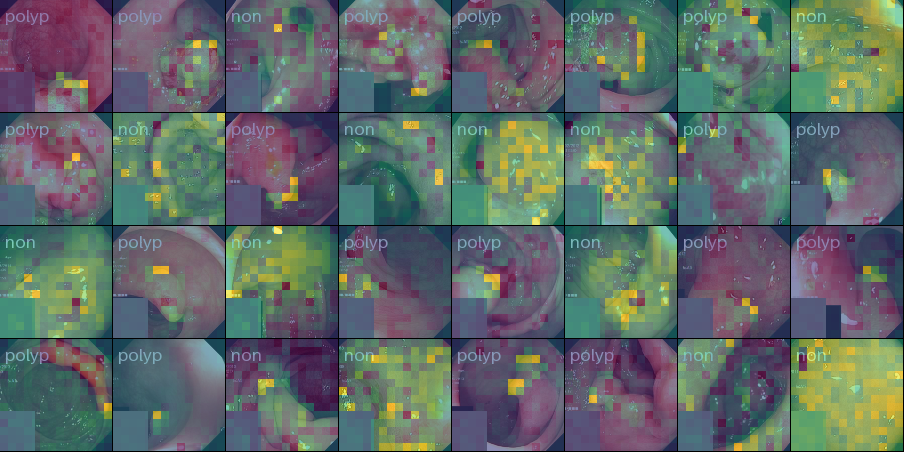
\includegraphics[scale=0.5]{./images/cropped_shap_gastro.png}
\caption{After cropping, the surrogate learns to focus on the true features}
\label{Shapley values for 196 players cropped gastro}
\end{figure}



Cropping of the images caused a considerable decrease of accuracy (see figure 
\ref{t:gastro_drop_accuracy}).



\begin{center}
\begin{tabular}{clSSSSS}
\toprule
% \multicolumn{2}{c}    {Trained Data}    &   

& Model & {ViT}  & {T2T\textunderscore ViT} &  {Swin} \\

\midrule
                &  non-cropped   & 93.7    &   94.9    &   98.3 \\
                &   cropped       &   89.2    &   89.8 & 89.1 \\

\midrule

\bottomrule
\label{t:gastro_drop_accuracy}
\end{tabular}
\end{center}


 


















\section{Evaluation of explanations}\label{s:evaluation}
Whereas in the previous sections we were interested mainly on the model performance and about how did they produce their output, here we focus rather on the explanations themselves. Before the explanations served us as a tool for checking the models' properties, here we would like to answer the question whether these explanations are the \textit{true} explanations. Namely, we would like to answer the following question: \textit{Are the features indicated by explanations as important indeed important for the model? Are the features indicated by explanations as not important indeed not important?}. These informal questions can be formalized in several ways and many metrics were proposed to evaluate the explanation methods, like monotonicity \cite{DBLP:journals/corr/abs-2007-07584}, max-sensitivity \cite{DBLP:conf/nips/YehHSIR19}, 
% faithfulness \cite{DBLP:conf/nips/Alvarez-
% MelisJ18} 
or ROAD \cite{DBLP:conf/icml/RongLBKK22}. 

The Shapley values are well-grounded theoretically, so they can serve as a baseline for other explanation methods, but only for the case of 16 players in which we have computed the Shapley values from scratch. For 196 players, we are interested in how the explainer model performs and whether it provides a better explanation than some commonly used methods like integrated gradients or saliency.





As it was already mentioned, HyperKvasir dataset provides the ground-truth segmentation masks that indicate where exactly are the polyps. Therefore, we can use these masks for the evaluation of the explanations. In the Figures 




\begin{figure}
\centering
\begin{subfigure}[b]{0.55\textwidth}
   
\includegraphics[width=1\linewidth]{./images/gastro_segmentation_1.png}
   \caption{}
   \label{fig:Ng1} 
\end{subfigure}

\begin{subfigure}[b]{0.55\textwidth}
   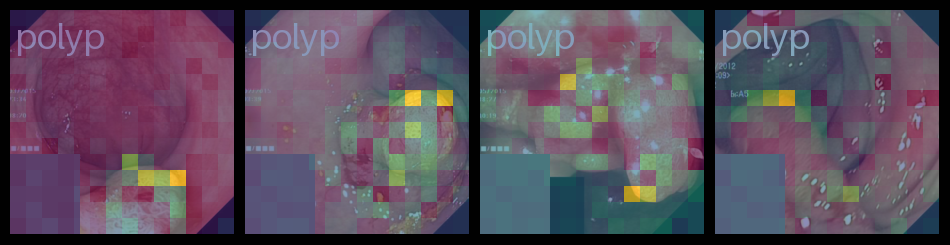
\includegraphics[width=1\linewidth]{./images/gastro_shap_for_segm_1.png}
   \caption{}
   \label{fig:Ng2}
\end{subfigure}

\caption[Two numerical solutions]{(a) Numerical solutions for the small-time system 
with a constant-curvature body shape showing the scaled leading-order veritcal 
reaction force $N_0$ versus the scaled body mass $M$ for various values of $g$. 
Again, $I=M$ for definiteness and $A=0.7$. (b) As for (a) but over a wider range of 
values of $M,I$.}
\end{figure}




We will discuss them in the following points.


\subsection{Monotonicity}
Like in the measuring of the models performance, evaluation of explanations should answer some meta-level questions which we would like to pose. For the monotonicity metric such a question is \textit{how imprecise would the prediction be if we did not know value of some feature?} \cite{DBLP:journals/corr/abs-2007-07584}. How much the model gets worse after removing a feature? More formally, let $a_1, \ldots, a_n$ be the feature attributions for a function (model) $f$ and $y^* = f(x^*)$ be the value of the model at some point $x^*$. We demand from the feature attribution $a_i$ that it satisfies the following equation:
\begin{equation} \label{monotonicity_equation}
    |a_i| \propto  \mathbb{E}\left(\textrm{loss}(y, f_i) | x_{-i}^*\right)  =  \int _{\chi _i} \textrm{loss} \left(y*, f_i(x_i)\right)p(x_i)dx_i ,
\end{equation}
where $f_i$ is the restriction of the function $f$ when all the coordinates apart from $x_i$ are fixed, $x^{∗}_{-i} = (x_1, \ldots, x_{i−1}, x_{i+1}, \ldots, x_N)$,
$\textrm{loss}$ is the loss function of interest and $\chi$ is the domain of $x_i$. The equation \ref{monotonicity_equation} describes mathematically a requirement that the attributions should be proportional to the performance of the model when the feature is removed. Note that this equation tries to omit the out-of-distribution problem: $x_i$ is not fixed or zeroed-out but we take an integral over $x_i$. However, this leads to another problem that some features cannot in reality occur together, like three-years old child with 2 metres height and thus some tuples $(x_1, \ldots x_i, \ldots x_N)$ may be unrealistic.


The \textit{monotonicity} is defined as the Spearman's correlation between the feature attributions and expected values from the equation \ref{monotonicity_equation}. More formally,

\begin{defi}
    The monotonicity for feature attributions $a_i$ is the Spearman’s correlation coefficient $\rho (a, e)$, where $a= \left(|a_1|, \ldots, |a_n|\right)$ is a vector containing the absolute values of the attributions and
    $e = \left(\mathbb{E}\left(\textup{loss}(y, f_1) | x_{-1}^*\right), \ldots \mathbb{E}\left(\textup{loss}(y, f_n) | x_{-n}^* \right) \right)$
contains the corresponding (estimated)
expectations, as computed in Equation \ref{monotonicity_equation}.
\end{defi}




\subsection{Max-sensitivity}
Sensitivity can be defined in a general way for a function $\Phi _f : \mathbb{R}^n \rightarrow \mathbb{R}^d$ (here subscript $f$ denotes that the function $\Phi$ depends on a function $f$) as a vector of partial derivatives:
\begin{equation}
    \left[ \nabla_{x} \Phi _{f}(x)\right]_j = \textrm{lim}_{\varepsilon \rightarrow 0} 
    \frac{\Phi _{f} (x + x \textbf{e}_{\textbf{j}} ) - \Phi_{f}(x)}
    {\varepsilon}.
\end{equation}
This equation measures how the function $\Phi _f$ changes as the input is varied infinitesimally.
In our setup, $\mathbb{R}^n$ is an input space of a model $f$ and $\Phi _f$ is the function which outputs the feature attributions for a given model. Sensitivity is a measure of how the feature attributions change after small changing of the model input. The idea behind this definition is that the attributions should not change much for similar inputs. To get rid of the potentially difficult to evaluate derivative, we can define max-sensitivity as follows:
\begin{defi}
    For an explanation function $\Phi _f $, a model $f$,  a given radius $r$, and a point $x$, max-sensitivity for explanation is given as:
    \begin{equation}
        \textup{SENS}_{\textup{MAX}} \left(\Phi _f, x, r \right) = \textup{max} _{|y-x| \leq r} \left\| \Phi _f(y) - \Phi _f(x)\right\|.
    \end{equation}
\end{defi}

This evaluation technique is tempting because it can be robustly estimated via Monte-Carlo sampling. However, it has two considerable drawbacks. Firstly, it is minimized simply for the constant function $\Phi$. Secondly, it is perhaps not relevant to demand small sensitivity from the feature attribution function. It can be an intrinsic characteristic of the model that it varies significantly for slightly changed inputs, and a good explanation should catch this behavior. Thus, max-sensitivity should rather not be used as the only evaluation method.


\subsection{ROAD}
The ROAD (RemOve And Debias) evaluation method was proposed in \cite{DBLP:conf/icml/RongLBKK22} as an improvement to the older method ROAR (RemOve And Retrain) \cite{DBLP:conf/nips/HookerEKK19}. The ROAR method measures how the accuracy of the model degrades when the features estimated as most important are removed. In order to avoid the out-of-distribution problem (inputs with removed features are from other distribution), ROAR proposes to retrain the model after removing important features. It is done for several percentages of important features: 10\%, 20\%, etc., so one should retrain the model several times. Note that the out-of-distribution problem is solved in a much less computationally expensive way via a surrogate model (see Section \ref{s:surrogate}) which is trained only once. 
The ROAD method proposes another way to reduce computations. It saves 99\% of the computational costs compared to ROAR. It also measures the accuracy after removing the most important features, but instead of retraining the model, it replaces the removed features with so-called noisy linear imputations. This method is based on the observation that pixels in the image (ROAD method is designed only for Computer Vision) are highly correlated. Intuitively, green pixels of the grass are, with a high probability, near other green grass pixels. One can for examplecheck that the correlation coefficient for direct neighbors in CIFAR-10 is $\rho=0.89$. Therefore, we have quite strong premises to suppose that each pixel can be approximated by the weighted mean of its neighbors with constant coefficients of a weighted mean:
\begin{align*}
    x_{i,j} &= w_{\textup{direct}} (x_{i,j+1} + x_{i,j−1} + x_{i+1,j} + x_{i−1,j} ) + \\
& w_{\textup{indirect}} (x_{i+1,j+1} + x_{i−1,j+1} + x_{i+1,j−1} + x_{i−1,j−1}),
\end{align*}
where $x_{i,j}$ are pixels and $w_{\textup{direct}}, w_{\textup{indirect}}$ are constant coefficients for direct and indirect (diagonal) neighbors of a pixel, respectively. The resulting system of equations can be efficiently solved even for a large number of missing pixels. This linear interpolation of removed pixels should not be learned by a model (otherwise the model could almost exactly reproduce the input) so there is added a small Gaussian noise.

In Figures \ref{ROAD_cifar_vit} - \ref{ROAD_cifar_swin} we present the accuracy of the models after removing the most important pixels according to the ROAD method. We can see that the accuracy on the batch of 32 images remains very high for the Saliency method even after removing 80\% of pixels. The explainer model outperforms it significantly. Removing the pixels marked as important by the explainer models causes quite an abrupt decrease in accuracy. We can also note that the accuracy for both Saliency and explainer feature attributions remains high for up to 20\% of removed pixels. It is probably due to the noisy linear imputations method. After removing only 20\% of pixels, the images remain very similar, though somewhat blurred.



\begin{figure}[H]
\centering
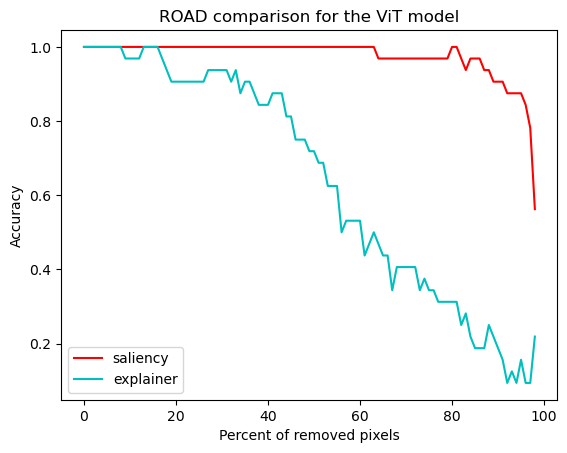
\includegraphics[scale=0.6]{./images/ROAD_cifar_vit.png}
\caption{ROAD metric for Saliency and explainer on CIFAR-10 dataset (ViT model)}
\label{ROAD_cifar_vit}
\end{figure}


\begin{figure}[H]
\centering
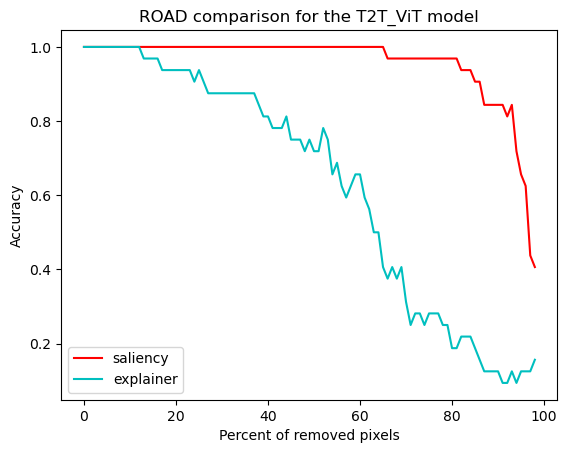
\includegraphics[scale=0.6]{./images/ROAD_cifar_t2t_vit.png}
\caption{ROAD metric for Saliency and explainer on CIFAR-10 dataset (T2T\textunderscore ViT model)}
\label{ROAD_cifar_t2t_vit}
\end{figure}


\begin{figure}[H]
\centering
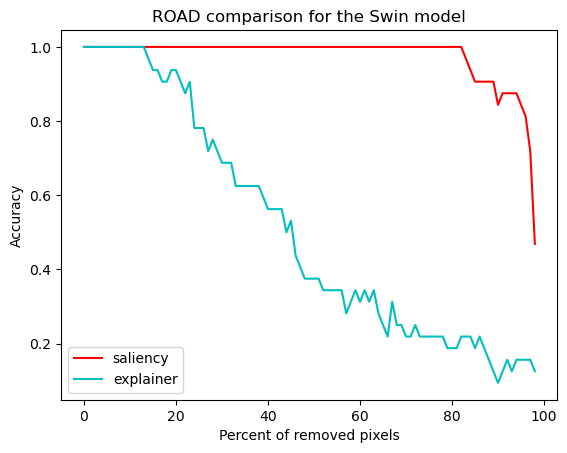
\includegraphics[scale=0.6]{./images/ROAD_cifar_swin.png}
\caption{ROAD metric for Saliency and explainer on CIFAR-10 dataset (Swin model)}
\label{ROAD_cifar_swin}
\end{figure}



The advantage of the Shapley values attributions over the Saliency method is even more visible when we compare the ROAD metrics computed for the HHyperKvasir dataset (see Figures \ref{ROAD_gastro_vit} - \ref{ROAD_gastro_swin}).


\begin{figure}[H]
\centering
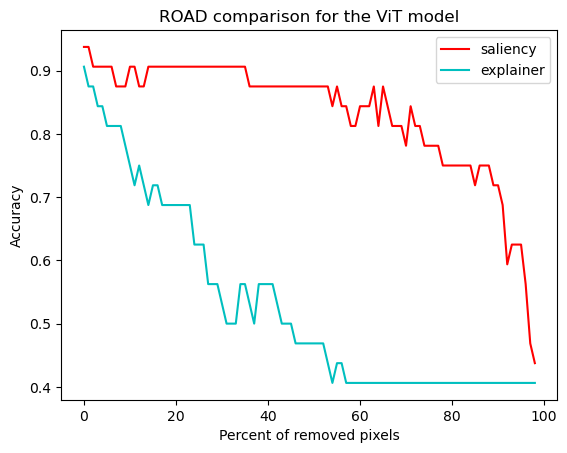
\includegraphics[scale=0.6]{./images/ROAD_gastro_vit.png}
\caption{ROAD metric for Saliency and explainer on HyperKvasir dataset (ViT model)}
\label{ROAD_gastro_vit}
\end{figure}


\begin{figure}[H]
\centering
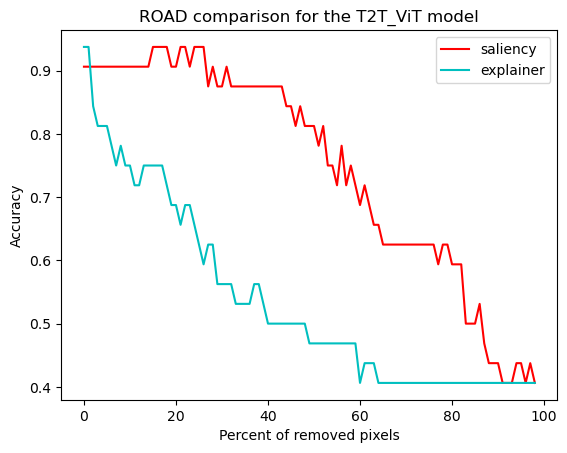
\includegraphics[scale=0.6]{./images/ROAD_gastro_t2t_vit.png}
\caption{ROAD metric for Saliency and explainer on HyperKvasir dataset (T2T\textunderscore ViT model)}
\label{ROAD_gastro_t2t_vit}
\end{figure}


\begin{figure}[H]
\centering
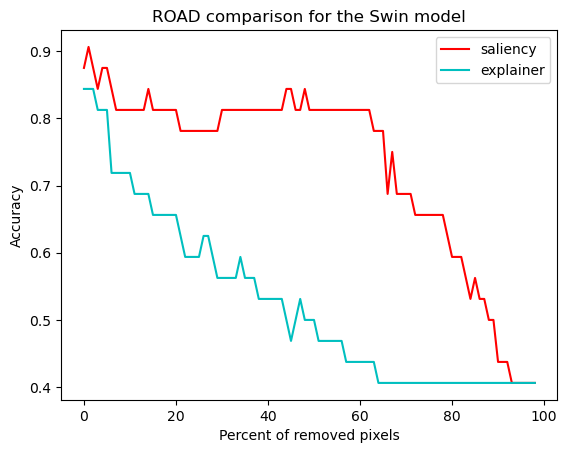
\includegraphics[scale=0.6]{./images/ROAD_gastro_swin.png}
\caption{ROAD metric for Saliency and explainer on HyperKvasir dataset (Swin model)}
\label{ROAD_gastro_swin}
\end{figure}










\subsection{Custom evaluation metric}

As it was already mentioned, the surrogate model solves the out-of-distribution problem connected with zeroing-out the pixels on the image. Therefore, to evaluate the explanations of the surrogate model, we can simply mask the pixels of the image. We have done it for several removing strategies (see Figure \ref{im: masked_shap_accuracy_vit}). Here we present the results for the CIFAR-10 dataset, later in this section we will provide the results for the HyperKvasir dataset.


% \begin{figure}[H]
% \centering
% 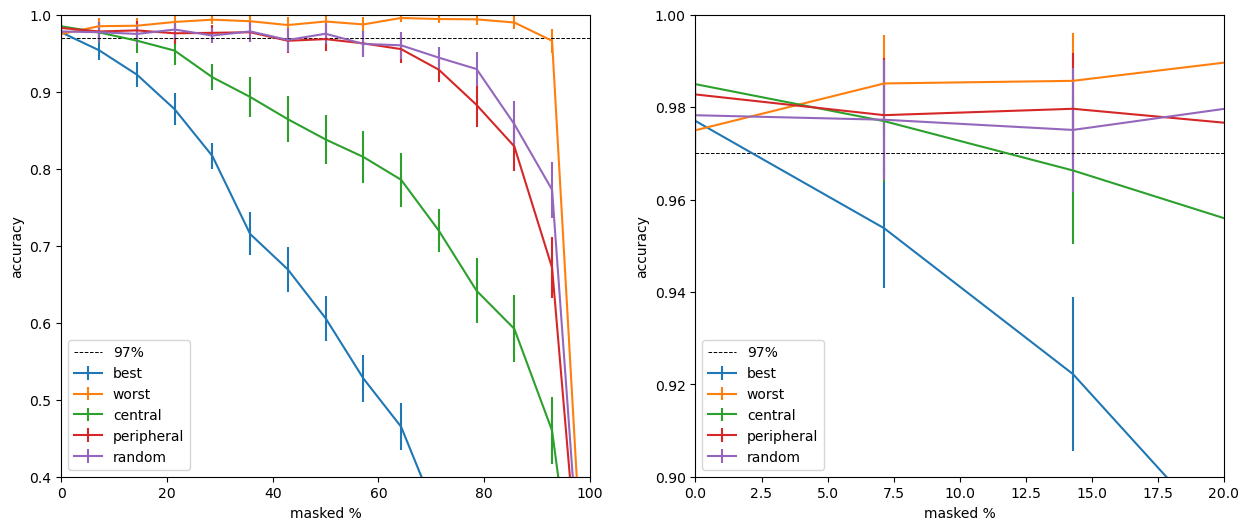
\includegraphics[scale=0.5]{./images/masking_explainer_patches_accuracy.png}
% \caption{Accuracy of the ViT surrogate model after zeroing out the given percentages of patches}
% \label{im: masked_shap_accuracy_vit}
% \end{figure}


We used five removal strategies: removing the best (most important) and worst (least important) patches according to Shapley values attributions, and also three independent methods: removing central, peripheral, and random patches. We can see that central features tend to be important for the model. However, the Shapley values computed by the explainer model detect even more important features and removing them causes a radical drop of accuracy. It is also worth noting that removing the worst features even increases the accuracy of the model. The explainer model detects patches that have a negative impact for the target class, and removing them increases the surrogate confidence for the target.

The Figure \ref{im: masked_shap_accuracy_vit} shows the accuracies of the ViT surrogate model. We present also the accuracies of the T2T\textunderscore ViT and Swin based surrogate models (Figures \ref{im: masked_shap_accuracy_t2t_vit}, \ref{im: masked_shap_accuracy_swin}).


% \begin{figure}[H]
% \centering
% 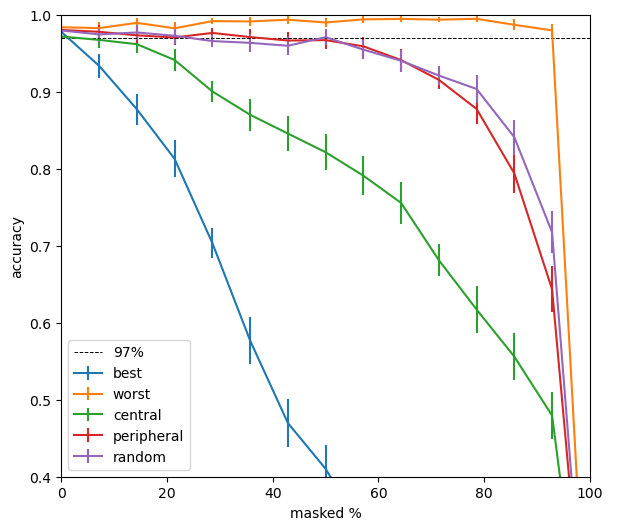
\includegraphics[scale=0.5]{./images/masking_explainer_patches_accuracy_t2t_vit_half-0.png}
% \caption{Accuracy of the T2T\textunderscore ViT surrogate model after zeroing out the given percentages of patches}
% \label{im: masked_shap_accuracy_t2t_vit}
% \end{figure}


% \begin{figure}[H]
% \centering
% 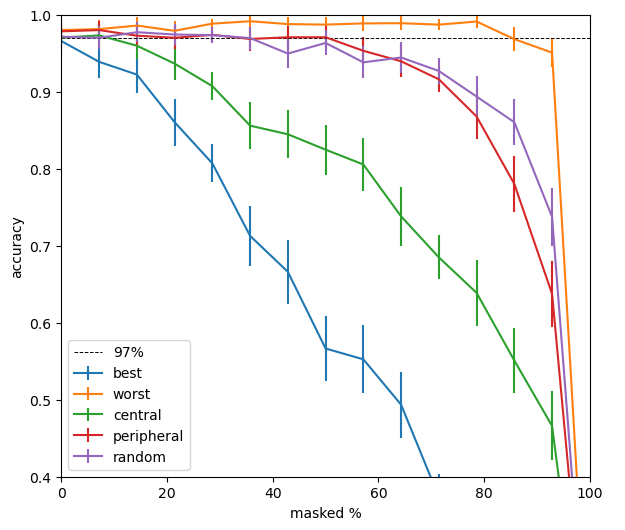
\includegraphics[scale=0.5]{./images/masking_explainer_patches_accuracy_swin_half-0.png}
% \caption{Accuracy of the Swin surrogate model after zeroing out the given percentages of patches}
% \label{im: masked_shap_accuracy_swin}
% \end{figure}

We can see that the T2T\textunderscore ViT model focuses the most on the local features. It strongly concentrates on the most important features, and thus it can perform well even if all patches apart from the most important are removed. On the other hand, the accuracy of T2T\textunderscore ViT drops the most rapidly after removing the most important features. The model which is the most robust to the removing of the most important features is Swin. It is probably due to its shifting strategy: the patches close to each other share the information, and removal of one feature is less harmful for the model performance.

On the Figure \ref{im: masked_saliency_accuracy_vit} we can see that the saliency attributions do not indicate the most important features with such precision as Shapley values. It confirms the results obtained for the ROAD metric. The accuracy after removing the least important features according to this metric is not only on par with the peripheral removing approach, but it is also worse than random removing. As for the most important patches according to this metric, it drops quite slowly, and the model obtains better accuracy after removing the best features than after removing simply central patches. It means that the saliency attributions do not properly recognize the importance of the patches.

\iftrue




\begin{figure}
\centering
\begin{subfigure}{.7\textwidth}
  \centering
  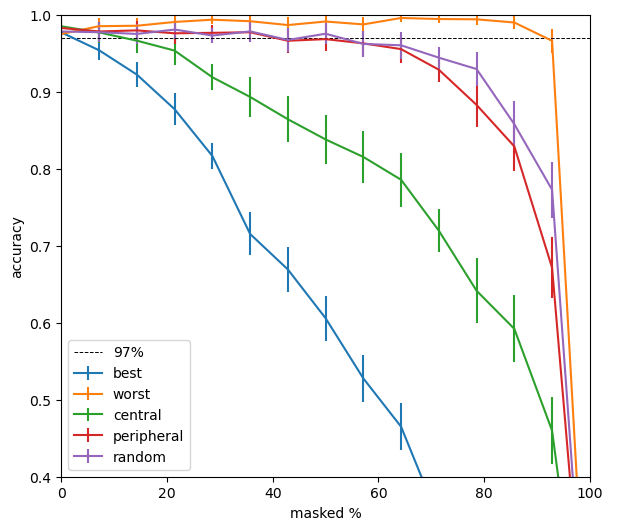
\includegraphics[width=.8\linewidth]{./images/masking_explainer_patches_accuracy_half-0.png}
  \caption{Explainer}
  \label{fig:sub1}
\end{subfigure}%
\begin{subfigure}{.7\textwidth}
  \centering
  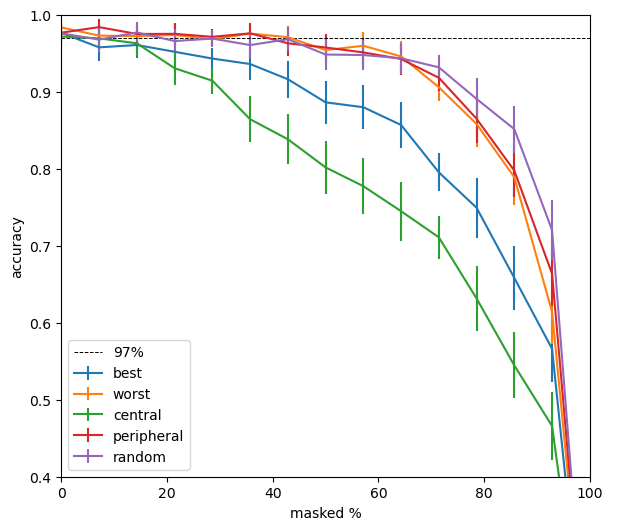
\includegraphics[width=.8\linewidth]
{./images/masking_saliency_patches_accuracy_vit_half-0.png}
  \caption{Saliency}
  \label{fig:sub2}
\end{subfigure}
\caption{Accuracy of the ViT surrogate model after removing features computed by explainer or saliency method}
\label{fig:ViT_Saliency_Explainer_CIFAR}
\end{figure}


\begin{figure}
\centering
\begin{subfigure}{.7\textwidth}
  \centering
  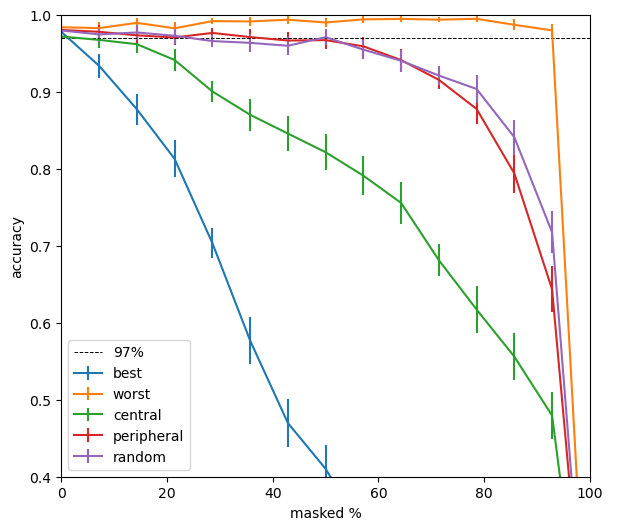
\includegraphics[width=.8\linewidth]{./images/masking_explainer_patches_accuracy_t2t_vit_half-0.png}
  \caption{Explainer}
  \label{fig:sub1}
\end{subfigure}%
\begin{subfigure}{.7\textwidth}
  \centering
  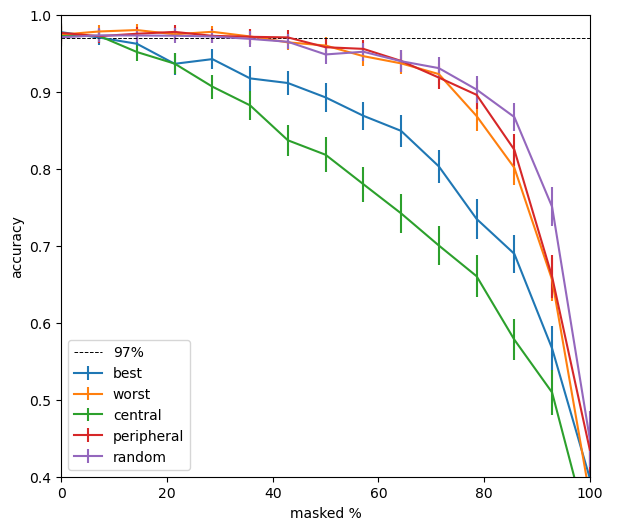
\includegraphics[width=.8\linewidth]
{./images/masking_saliency_patches_accuracy_t2t_vit_half-0.png}
  \caption{Saliency}
  \label{fig:sub2}
\end{subfigure}
\caption{Accuracy of the T2T\textunderscore ViT surrogate model after removing features computed by explainer or saliency method}
\label{fig:T2T_ViT_Saliency_Explainer_CIFAR}
\end{figure}


\begin{figure}
\centering
\begin{subfigure}{.7\textwidth}
  \centering
  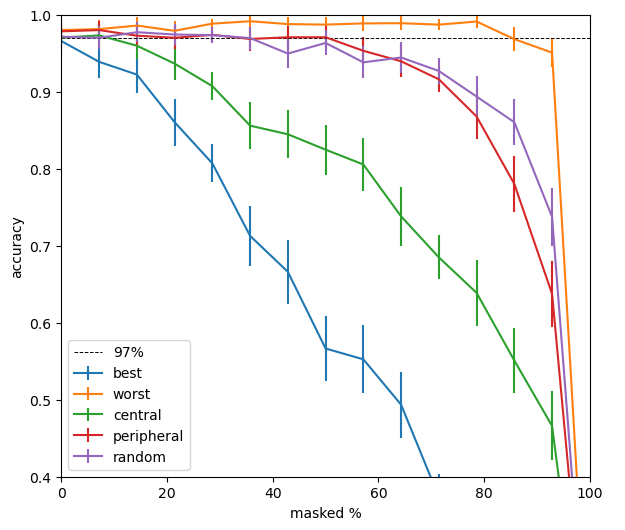
\includegraphics[width=.8\linewidth]{./images/masking_explainer_patches_accuracy_swin_half-0.png}
  \caption{Explainer}
  \label{fig:sub1}
\end{subfigure}%
\begin{subfigure}{.7\textwidth}
  \centering
  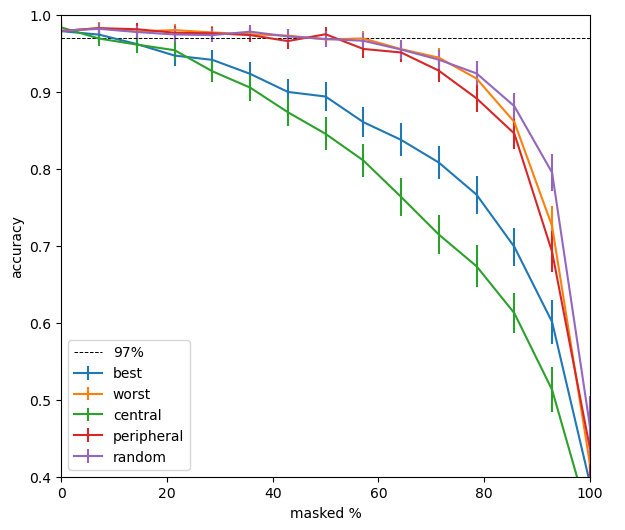
\includegraphics[width=.8\linewidth]
{./images/masking_saliency_patches_accuracy_swin_half-0.png}
  \caption{Saliency}
  \label{fig:sub2}
\end{subfigure}
\caption{Accuracy of the Swin surrogate model after removing features computed by explainer or saliency method}
\label{fig:Swin_Saliency_Explainer_CIFAR}
\end{figure}







The results for the HyperKvasir dataset show even better the advantages of the Shapley values computed by the explainer model over the Saliency method (see Figures \ref{ViT_Saliency_Explainer_HyperKvasir} -\ref{Swin_Saliency_Explainer_HyperKvasir}). We can see that removing the patches recognized as important for the prediction by the Saliency method causes a similar drop in accuracy to the random removing approach. As a matter of fact, all the curves for the Saliency method look similar, and methods of removing the patches change the accuracy in a similar way. 

On the other hand, explainer recognizes the important features very precisely, so that the accuracy after removing the most important features drops fastly for all the three models (ViT, T2T\textunderscore ViT, and Swin). Worst, peripheral, and central removing approaches of removing give the curves that lie between the curves for the worst and best patches removing approaches, as we expect from a proper feature attribution method.








\begin{figure}
\centering
\begin{subfigure}{.7\textwidth}
  \centering
  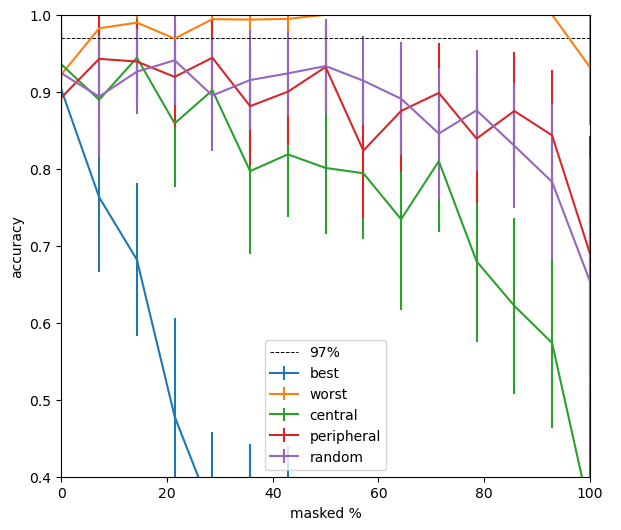
\includegraphics[width=.8\linewidth]{./images/vit_gastro_masking_explainer_patches_accuracy_half-0.png}
  \caption{Explainer HyperKvasir}
  \label{fig:sub1}
\end{subfigure}%
\begin{subfigure}{.7\textwidth}
  \centering
  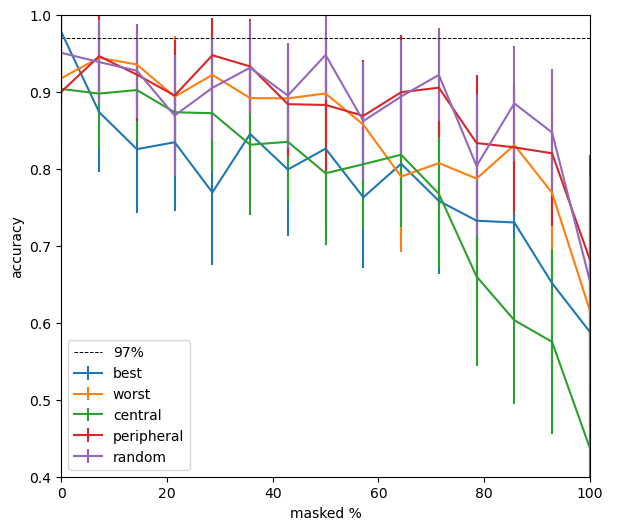
\includegraphics[width=.8\linewidth]
{./images/vit_gastro_masking_saliency_patches_accuracy_half-0.png}
  \caption{Saliency HyperKvasir}
  \label{fig:sub2}
\end{subfigure}
\caption{Accuracy of the ViT surrogate model after removing features computed by explainer or saliency method}
\label{fig:ViT_Saliency_Explainer_HyperKvasir}
\end{figure}












\begin{figure}
\centering
\begin{subfigure}{.7\textwidth}
  \centering
  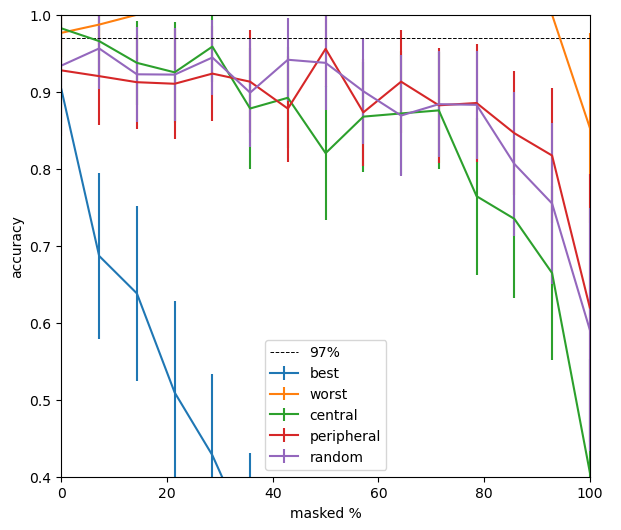
\includegraphics[width=.8\linewidth]{./images/t2t_vit_gastro_masking_explainer_patches_accuracy_half-0.png}
  \caption{Explainer HyperKvasir}
  \label{fig:sub1}
\end{subfigure}%
\begin{subfigure}{.7\textwidth}
  \centering
  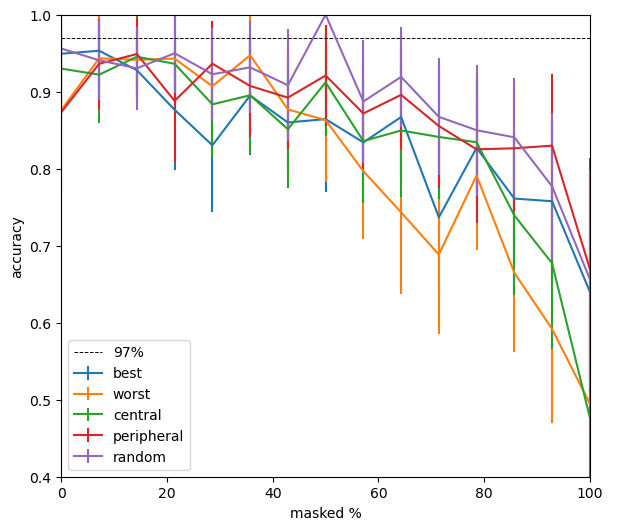
\includegraphics[width=.8\linewidth]
{./images/t2t_vit_gastro_masking_saliency_patches_accuracy_half-0.png}
  \caption{Saliency HyperKvasir}
  \label{fig:sub2}
\end{subfigure}
\caption{Accuracy of the T2T\textunderscore ViT  surrogate model after removing features computed by explainer or saliency method}
\label{fig:T2T_ViT_Saliency_Explainer_HyperKvasir}
\end{figure}
















\begin{figure}
\centering
\begin{subfigure}{.7\textwidth}
  \centering
  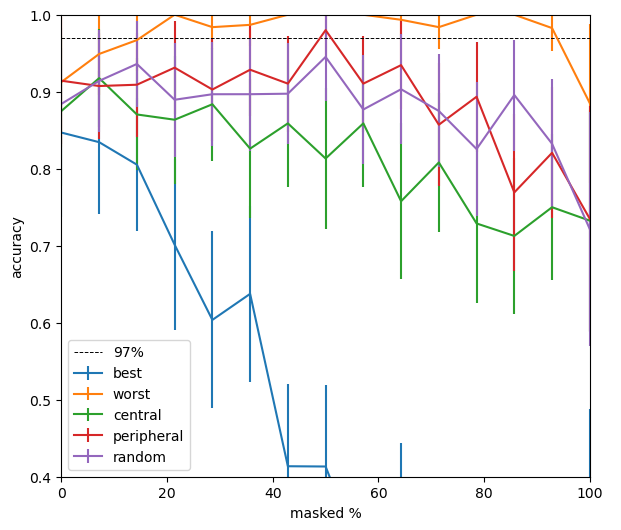
\includegraphics[width=.8\linewidth]{./images/swin_gastro_masking_explainer_patches_accuracy_half-0.png}
  \caption{Explainer HyperKvasir}
  \label{fig:sub1}
\end{subfigure}%
\begin{subfigure}{.7\textwidth}
  \centering
  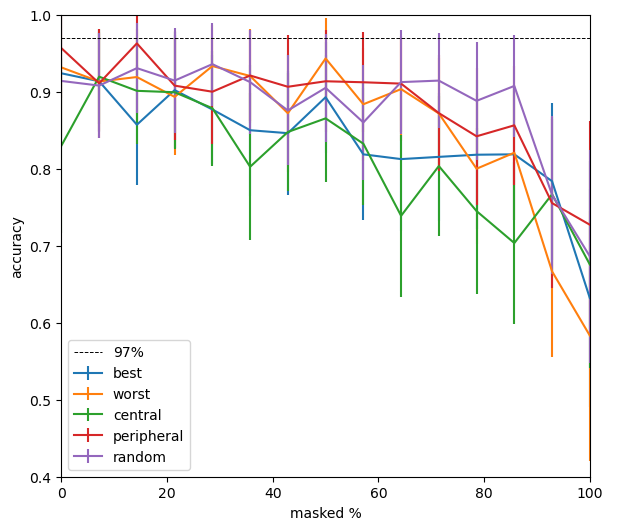
\includegraphics[width=.8\linewidth]
{./images/swin_gastro_masking_saliency_patches_accuracy_half-0.png}
  \caption{Saliency HyperKvasir}
  \label{fig:sub2}
\end{subfigure}
\caption{Accuracy of the Swin surrogate model after removing features computed by explainer or saliency method}
\label{fig:Swin_Saliency_Explainer_HyperKvasir}
\end{figure}






























\begin{figure}[H]
\centering
\includegraphics[scale=0.5]{./images/vit_surrogate_masks.png}
\caption{Vit surrogate model}
\label{vit_surrogate_masks}
\end{figure}


\begin{figure}[H]
\centering
\includegraphics[scale=0.5]{./images/t2t_vit_surrogate_masks.png}
\caption{T2T\textdel after removing features computed by explainer or saliency methodscore vit surrogate model}
\label{t2t_vit_surrogate_masks}
\end{figure}


\begin{figure}[H]
\centering
\includegraphics[scale=0.5]{./images/swin_surrogate_masks.png}
\caption{Swin surrogate model}
\label{swin_surrogate_masks}
\end{figure}






\begin{figure}[H]
\centering
\includegraphics[scale=0.5]{./images/vit_classifier_masks.png}
\caption{Vit classifier model}
\label{vit_classifier_masks}
\end{figure}


\begin{figure}[H]
\centering
\includegraphics[scale=0.5]{./images/t2t_vit_classifier_masks.png}
\caption{T2t\textdel after removing features computed by explainer or saliency methodscore vit surrogate model}
\label{t2t_vit_classifier_masks}
\end{figure}


\begin{figure}[H]
\centering
\includegraphics[scale=0.5]{./images/swin_classifier_masks.png}
\caption{Swin classifier model}
\label{swin_classifier_masks}
\end{figure}




\fi


















\printbibliography

\end{document}


%%% Local Variables:
%%% mode: latex
%%% TeX-master: t
%%% coding: latin-2
%%% End:
